\documentclass[12pt, a4paper, twoside, openright]{book}

\usepackage{vuwthesis} % sets up some local things, mostly the front page

%\usepackage{palatino} % sets palatino as the default font
\usepackage{fontspec}
\setmainfont{TeX Gyre Pagella}
\usepackage{url} % for typesetting urls

\usepackage[colorlinks=true, linkcolor=black, urlcolor=black,citecolor=black]{hyperref}

\usepackage{xspace}
\usepackage{graphicx}
\usepackage{caption}
\usepackage{subcaption}
\usepackage{siunitx}
\usepackage[table]{xcolor}
\usepackage[bottom=3.0cm, left=3cm, right=3.0cm]{geometry}

\usepackage{pdflscape}
%\renewcommand{\baselinestretch}{1.00}


\newcommand{\Ttwo} {\textit{T\textsubscript{2}}\xspace}
\newcommand{\SOtwo} {\textit{sO\textsubscript{2}}\xspace}
\newcommand{\TtwoO} {\textit{T\textsubscript{20}}\xspace}
\newcommand{\Kzero} {\textit{K\textsubscript{0}}\xspace}
\newcommand{\Gzero} {\textit{G\textsubscript{0}}\xspace}
\newcommand{\Otwo} {O\textsubscript{2}\xspace}
\newcommand{\Ntwo} {N\textsubscript{2}\xspace}
\newcommand{\COtwo} {CO\textsubscript{2}\xspace}
\newcommand{\TR} {\textit{T\textsubscript{R}}\xspace}
\newcommand{\Texc} {\textit{τ\textsubscript{ex}}\xspace}
\newcommand{\rc} {\textit{r\textsubscript{c}}\xspace}
\newcommand{\Tech} {\textit{t\textsubscript{ec}}\xspace}
\newcommand{\Rtwo} {\textit{R\textsubscript{2}}\xspace}
\newcommand{\Bzero} {\textit{B\textsubscript{0}}\xspace}
\newcommand{\Bone}  {\textit{B\textsubscript{1}}\xspace}
\newcommand{\Ttwostar} {\textit{T\textsubscript{2}\**}\xspace}
\newcommand{\Tone} {\textit{T\textsubscript{1}}\xspace}
\newcommand{\Hct} {\textit{Hct}\xspace}

\sisetup{separate-uncertainty = true}
%\sisetup{unit-color = blue}
%\sisetup{number-color = blue}

\begin{document}

\frontmatter
% Book style knows about front matter
% Report style doesn't so you need to set roman numbering etc yourself :-(

%%%%%%%%%%%%%%%%%%%%%%%%%%%%%%%%%%%%%%%%%%%%%%%%%%%%%%%
\title{Parameter Space Mapping for Blood Oxygenation Measurement with Low Field NMR}
\author{Dion Gary Thomas}

\subject{Physics}
\abstract{
Blood oxygenation is a critical physiological parameter for patient health.
The clinical importance of this parameter means that measurement of blood oxygenation is a routine part of care.
Magnetic resonance provides a way to measure blood oxygenation through the paramagnetic effect of deoxy-haemoglobin, which decreases the \Ttwo relaxation time of blood.
This effect has been well characterised at high fields (\SI{>1.5}{T}) for use in Magnetic Resonance Imaging, and it is a contributing factor to the Blood Oxygenation Level Dependent contrast used in functional MRI.
However there are relatively few studies of this effect at low magnetic fields, and these have only looked at extreme levels of oxygenation/deoxygenation.
To study this effect for potential application in a low-field device, we measured this effect to determine how factors such as oxygenation, field strength and CPMG echo time affect the \Ttwo of blood.

A continuous flow circuit, similar to a cardiopulmonary bypass circuit, was used to control parameters such as oxygen saturation and temperature, before the blood sample flowed into a variable field magnet (set at fields between 5-40 MHz), where a series of CPMG experiments with echo times ranging from \SIrange{1}{20}{ms} were performed to measure the \Ttwo.
Additionally, the oxygen saturation was continually monitored by an optical sensor, for comparison with the \Ttwo changes.
This allowed us to test the sensitivity of this effect at low fields.

These results show that at low fields, the \Ttwo relaxation change still follows the trends shown in the literature, with a dependence on \Bzero squared, and on the fraction of deoxyhaemoglobin squared.
Additionally, these results were also compared with two theoretical models for the dependence on echo time, which have previously been tested at high fields: the Luz-Meiboom equation, and the Jensen and Chandra model.
Both models gave good agreement with the data measured at low fields.
These experiments show that the \Ttwo changes in blood due to oxygenation are still visible at low field, and that this technique should be feasible in a low field device.


%Changes in blood oxygen saturation change the magnetic properties of red blood cells, generating an inhomogeneous magnetic field which decreases the \Ttwo relaxation time of the water protons in blood.
%This effect has been well characterised at imaging fields (\SI{>1.5}{T}), and has been applied to measure changes in blood oxygen saturation \textit{in-vivo}, but at the low fields required for portable NMR devices, there are only a handful of studies in the literature.
%These showed that the size of the \Ttwo change increases with the field strength squared, althuoguh these experiments at low fields only looked at extreme levels of oxygenation/deoxygenation.

%At these field strengths and echo times, both models provided good agreement with the experimental data, however the Jensen and Chandra model model was able to provide better fits to the data.
}
% Books don't normally have abstracts, and this is a bit of a hack

% Uncomment the appropriate degree
%\phd
\mscthesisonly
%\mscwithhonours
%\mscbothparts
% \otherdegree{DEGREE OR DIPLOMA NAME}



%%%%%%%%%%%%%%%%%%%%%%%%%%%%%%%%%%%%%%%%%%%%%%%%%%%%%%%
\hypersetup{pdftitle=\@title}



\maketitle

\chapter*{Acknowledgments}\label{ch:ack}
Firstly I need to thank my supervisors: Sergei Obruchkov, Shieak Tzeng and Petrik Galvosas for their excellent supervision, and for giving me the opportunity to pursue this research.
In particular I would like to thank them for their encouragement when the baby-MRI decided to choke a month before I was due to give a talk about results collected on it.
I would like to think that the panic and stress that caused was worth it.

Another big thanks goes to the other members and friends of the VUW NMR group over the last 2 years.
Thank you for making this such a fun place to work, and for all of your help and friendship.
To my other past supervisors, Marcel and Tim, thank you for introducing me to NMR and for letting me spend my honours year here.

Next, I would like to thank my fantastic friends and flatmates.
Thanks to them for putting up with my work stories, and for helping to keep me sane.
Of course, I must also thank Wilbur, who is somehow always excited to see me get home.

I would not have been able to complete this work without the care and support I have received from my family.
Thanks to my Mum and Dad for their encouragement, advice and support, and for treating me to weekend brunches.
And to my brother Adrian for his motivated assistance in acquiring research materials.
Thanks also to my family in the Philippines, especially my Lola, for their support and prayers.

I gratefully acknowledge funding support from the New Zealand Ministry of Business, Innovation and Employment, and the Australian and New Zealand Society for Magnetic Resonance for a travel grant to present this work at the ANZMAG conference.

I look forward to more experimenting in the future

\addtocontents{toc}{\vskip-1.0cm}

\tableofcontents

\listoffigures
\listoftables
%%%%%%%%%%%%%%%%%%%%%%%%%%%%%%%%%%%%%%%%%%%%%%%%%%%%%%%

% book style knows about mainmatter
% if you are using report style you will have to rest page numbering etc.
\mainmatter

%%%%%%%%%%%%%%%%%%%%%%%%%%%%%%%%%%%%%%%%%%%%%%%%%%%%%%%

% individual chapters included here

\chapter{Introduction}\label{ch:intro}

Blood oxygenation is a critical parameter for assessing patient health and the management of disease.
Oxygen saturation measurement are a routine part of care, and changes in these measurements can act as warning signs of acute/serious problems in the body.
Low levels of Oxygen can cause tissue damage and cell death, particularly in sensitive tissue such as the brain, where even brief periods of
hypoxia can have catastrophic effects.
Low Oxygen levels can also be an issue for neonates, who can have circulatory and pulmonary systems which are still developing.
Being able to detect changes in oxygenation quickly means that action can be taken to limit and/or prevent ill effects to patients.

The typical method for measuring blood oxygenation in patients is through pulse oximetry, a non-invasive method which measures the change in absorbance at
various wavelengths of light to detect the presence of oxygenated and deoxygenated haemoglobin.
This method can produce quick measurements of the blood oxygen saturation, while also being relatively cheap and robust.
Because it measures the blood, this technique provides information about Oxygen saturation across the whole body, measured at a single point on the finger or ear lobe.
However, this means that these saturations are not necessarily representative of Oxygen levels in specific parts of the body, such as the brain.
An example is given by TODO if there are issues with blood flow to specific areas (ischemia?), these will not necessarily be reflected by pulse oximetry.
Because of this, local tissue oxygenation measurements are desired by physicians, but they are difficult to measure.

Techniques for measuring local tissue oxygenation in the brain include the use of NIRS (Near-Infrared Spectroscopy), and the use of oxygen measuring
polarographic electrodes.
NIRS is a non-invasive method where the changes in light absorption from oxy/deoxy-haemoglobin are observed at near-infrared wavelengths, which can penetrate
into tissue, similar to pulse oximetry.
This technique is commercially available and already used regularly, particularly for monitoring neonates.
However, it can be difficult to measure the local oxygenation of deeper structures, as it depends on light traveling through the tissue and returning to the sensor.
Oxygen electrodes can also be used, which can be inserted into the desired area for measurement.
These give a direct readout of the p\Otwo, in the tissue surrounding the probe.
However, inserting these oxygen electrodes into the tissue is extremely invasive, which has limited the use of these sensors.

Nuclear Magnetic Resonance (NMR) presents an alternative way to measure blood oxygen saturation.
It has been known since the early 1980s that the saturation of blood is linked to it's transverse relaxation time \Ttwo.
This relationship is caused by the change in the magnetic properties of haemoglobin when bound to oxygen.
This effect is a contributing factor to BOLD(Blood Oxygen Level Dependent) contrast which underlies fMRI(functional Magnetic Resonance Imaging).
Non-invasive measurement of local oxygen saturation has also been demonstrated using this effect.
These applications have been developed using high-field (>1.5 T) imaging systems, whose large size and cost means that these techniques are not in clinical use.

In the last 25 years, developments in portable magnetic resonance, using single sided magnets and coils, have meant that NMR can be used outside of laboratories and MRI suites.
These magnetic resonance instruments produce a sweet spot, where the magnetic field and coil sensitivity combine to produce an NMR signal from protons inside this region.
Combining this with the oxygen dependent \Ttwo change could produce an instrument which is sensitive to local changes in tissue oxygenation.
However, single sided NMR systems have limitations on the strength and homogeneity of the magnetic field they produce, due to the use of permanent magnets, and the geometry of the system.
This means that it is important to understand how factors like field strength and homogeneity affect how oxygenation dependent \Ttwo changes can be observed in this type of system.

%Additionally, the magnitude of the change in oxygen saturation that can be detected using this magnetic resonance relaxation effect is also important, as being able to measure slight changes in oxygenation will mean that this technique can provide clinically relevant early warnings of low oxygenation.

\section{NMR Measurement of oxygen saturation}
The effect of \SOtwo on the \Ttwo of blood was originally described by \cite{ThulbornOxygenationdependencetransverse1982} in 1982, who investigated how \Ttwo changed as a function of oxygenation, magnetic field strength and haematocrit (fraction of blood in red blood cells.
Thulborn found that the \Rtwo ($\mathit{\frac{1}{T_2}}$) of blood decreased with $(100-\mathit{SO_2})^2$.
Using a variety of spectrometers and NMR systems, he also showed that the strength of this effect scales with \Bzero squared, and that this effect requires that the red blood cells are intact (as no change in \Ttwo occured when the cells were lysed.)

From this initial study, other researchers studied how the effect can be detected at lower fields.
Gomori measured the \Ttwo of samples of oxygenated and deoxygenated blood at fields ranging from \SIrange{0.19}{1.4}{T}, and found that changes were still visible at these lower fields\cite{GomoriNMRRelaxationTimes1987}.
This sort of experiment was also completed by Brooks, who found that \Ttwo shortening were visible at fields between \SIlist{0.05;1.5}{T} \cite{BrooksComparisont2relaxation1995}.
Brooks mapped out the dependence on field strength more finely than Gomori, and was able to show that the size of the effect still scales with \Bzero squared at low fields.
In these studies, the samples of blood were measured with either completely oxygenated and completely deoxygenated blood, typically obtained by
There are a handful of other studies of this effect at these low field strengths, such as \cite{BryantMagneticrelaxationblood1990} and Stadelmann\cite{StadelmannRelaxationtimesvenous1991},
although like the studies by Brooks and Gomori, these were only done using samples of deoxygenated and oxygenated blood.

More recently, this effect has been studied \textit{in-vitro} for applications in high field imaging systems (\SI{>1.5}{T}.)
Silvennoin\cite{JohannaSilvennoinenBloodNMRrelaxation2002}, Stefanovic\cite{StefanovicHumanwholebloodrelaxometry2004}, Chen\cite{ChenHumanwholeblood2009} and Gardener\cite{GardenerDependencebloodR22010} scanned samples with varying oxygenation levels in MRI scanners (1.5, 2.35, 3 or 4.7 T) to study the change in \Ttwo as a function of oxygenation, haematocrit and CPMG echo time.
These studies showed that the effect follows the same quadratic trend found by Thulborn, and shows good agreement with the theoretical models discussed in \autoref{ch:models}.

Another method of studying \Ttwo changes with \SOtwo \textit{in-vitro} was described by Meyer et al., who used a continuous flow loop to measure \Ttwo at varying levels of \SOtwo, with a spectrometer at \SI{4.7}{T}.
This method was more recently used by the group of Peter van Zilj, who has published multiple studies (\cite{ZhaoOxygenationhematocritdependence2007,GrgacTransversewaterrelaxation2017,QinDeterminationwholebrainoxygen2011} on the dependence of \Ttwo on \SOtwo, haematocrit, and on field strength.
These studies have looked at magnetic field strengths from \SIrange{3.0}{16.4}{T}.

The effect on \Ttwo of \SOtwo has also been applied in \textit{in-vivo} imaging, with a pioneering study by Wright\cite{WrightEstimatingoxygensaturation1991}, who measured changing oxygen saturation in the body using \Ttwo changes.
More recently, other researchers have developed methods for imaging \SOtwo in blood based on this \Ttwo effect.
TRUST-MRI (\Ttwo Relaxation Under Spin Tagging) can be used to measure the \Ttwo of blood, and convert this into an \SOtwo using a calibration curve \cite{LuQuantitativeevaluationoxygenation2008}.
Measurement of oxygenation using \Ttwo values collected with different echo times has also been demonstrated \cite{VargheseCMRbasedbloodoximetry2017}.
While these methods provide good agreement with other measurements of \SOtwo, they are not typically used in clinical practice.

In this thesis, this parameter space has been mapped out to determine how field strength, CPMG echo time, and other factors affect the magnitude of the oxygenation
\Ttwo effect in whole blood.
\autoref{ch:background} presents background information on NMR relaxation, and on the origin of the oxygenation dependent \Ttwo change.
\autoref{ch:exptsetup} describes the two versions of the experimental setup used for the two series of experiments in this thesis.
\autoref{ch:stoppedflow} presents the results of stopped flow experiments into the \Ttwo change at a series of oxygenation steps, while \autoref{ch:cont} presents the results of experiments measuring \Ttwo changes continuously as \SOtwo is slowly decreased.
\autoref{ch:models} evaluates an alternative model proposed by Jensen and Chandra to describe the process causing decreases in \Ttwo\cite{JensenNMRrelaxationtissues2000}.

\chapter{Background}\label{ch:background}

\section{Nuclear Magnetic Resonance}

Nuclear Magnetic Resonance (NMR) is an effect most often associated with chemical spectroscopy, or magnetic resonance imaging.
This section will give a brief overview of the physics of NMR, using the semi-classical model and the Bloch equations.
It describes NMR occuring to protons (\textsuperscript{1}H), which is the most common nucleus used for NMR and what is used in this thesis, although NMR can be observed with any nuclei with non-zero spin.
For a more complete discussion, the reader is directed to one of the many textbooks on the subject, including books by Abragham\cite{AbragamPrinciplesNuclearMagnetism1961} and Callaghan\cite{CallaghanPrinciplesNuclearMagnetic1994} or Brown et al.\cite{BrownMagneticResonanceImaging2014a}.

Protons have an magnetic moment due to their intrinsic angular momentum, or `spin'.
To observe nuclear magnetic resonance, protons are put into a magnetic field (\Bzero) that interacts with the protons magnetic moment, lowering the energy of magnetic moments aligned with \Bzero (along \textit{z}).
This makes it more energetically favourable for the protons' magnetic moment to align with the field, so that slightly more protons are aligned with the field.
This imbalance generates a net magnetisation aligned with the magnetic field, which is manipulated with the \textit{B\textsubscript{1}} field to generate the magnetic resonance signal.
As the size of the net magnetisation depends on the relative difference of spins towards and against the field, the net magnetisation becomes stronger when a larger \Bzero field is used.
Any imbalance created is typically very small, which means that the NMR signal generated is very weak.

A magnetic moment in a magnetic field experiences a torque, which causes it to rotate around an axis along the magnetic field.
This is called Larmor precession, and gives rise to the Larmor frequency $\omega$, which defines the rate of rotation.
Protons in a magnetic field precess at a frequency given by \autoref{eq:back-larmor}, where $\gamma$ is the gyromagnetic ratio (\SI{2.56e8}{rad/T} for protons).
\begin{equation}
\omega = \gamma B_0
\label{eq:back-larmor}
\end{equation}
At equilibrium, the net magnetisation is along \textit{z}, so precession is not visible.

The effect of the \Bone field can be seen by considering a frame (\textit{x', y', z'}) which rotates around the \textit{z} axis at this precession frequency (a `rotating frame', when compared to the stationary `lab frame')
In the rotating frame, the net magnetisation still lies along the \textit{z}-axis.
Applying an additional magnetic field, along \textit{x'} (i.e. perpendicular to \Bzero) to the \textit{z}-axis causes the magnetisation to rotate around \textit{x'} towards \textit{y'}, following the same precession principle.
The strength and time that the\Bone field is applied for can be changed to control the amount of rotation, leading to \SI{90}{\degree} and \SI{180}{\degree} pulses.

Transforming this into the lab frame means that the \Bone field becomes a magnetic field oscillating at the Larmor frequency,
while the components of the magnetisation along \textit{x} and \textit{y} correspond to a rotating magnetisation in the sample.
This produces the resonance condition for NMR -- the frequency of the \Bone field needs to match the precession frequency to cause maximum rotation.
These can be created and detected using a coil, as the rotating magnetic field from the sample induces a voltage in the coil due to Faraday's Law.
This NMR signal is known as the Free Induction Decay (FID).

\section{\Tone and \Ttwo relaxation}
The NMR signal from a sample decays due to relaxation with two main mechanisms.
It can be caused by the return of net magnetisation to equilibrium, or by a loss of coherence across a sample.

As mentioned above, the equilibrium state of a sample in a \Bzero field is for the net magnetisation to align with the \Bzero magnetic field.
When this is disturbed, for example, in an NMR experiment or when the sample is first placed in the \Bzero field, the protons in the sample exchange energy to return to the equilibrium.
This process, also known as spin-lattice relaxation, is described by \autoref{eq:back-Tone}, where M\textsubscript{0} is the equilibrium magnetisation, and the time constant for relaxation is \Tone.

\begin{equation}
\frac{\mathrm{d} M_z}{\mathrm{d} t} = \frac{1}{T_1} (M_0-M_z)
\label{eq:back-Tone}
\end{equation}

The \Tone of a sample can be determined by an inversion recovery experiment.
A \SI{180}{\degree} pulse is applied to the sample, and the magnetisation remaining is measured after a range of variable delay time ($t_d$ )by applying a \SI{90}{\degree} pulse and taking the intensity of the FID.
This can be used to fit a curve with the equation
\begin{displaymath}
M(t_d) = M_0 (1 - 2 e^{-frac{t_d}{T_1}})
\end{displaymath}

In most cases, the \Tone controls how rapidly an experiment can be repeated.
A general rule is to set the repetition time (\TR - the delay between experiments) to 5$\times$\Tone, so that the sample magnetisation recovers to \SI{>99}{\percent} of its original equilibrium level.
Otherwise the signal produced will be weaker, as it depends on the magnetisation along the \textit{z} axis.
This also removes any remaining transverse magnetisation, as the protons return to equilibrium.
Because of this, \Ttwo < \Tone.

The \textit{x} and \textit{y} components of a sample's magnetisation (transverse magnetisation) also undergoes relaxation.
The transverse magnetisation is generated by the combination of magnetisation from protons across the sample.
The NMR signal is generated when the magnetic moments of all of the protons in a sample precess at the same rate, and are all aligned in the same direction (i.e. have the same phase), creating coherence.
If protons in part of the sample experience a different magnetic field, they precess at a different rate and lose coherence with the rest of the sample.
This reduces the overall transverse magnetisation of the sample, which decreases following \autoref{eq:back-Ttwo}, where \Ttwo is the time constant for this relaxation.

\begin{equation}
\frac{\mathrm{d}M_{xy}}{\mathrm{d}t} = - \frac{1}{T_2} (M_{xy})
\label{eq:back-Ttwo}
\end{equation}

In a physical sample, protons are always experiencing different magnetic fields due to the fluctuating magnetic moments of surrounding protons.
This process of dephasing is random and non-reversible.
The physical properties of a sample control the amount of interaction between protons on surrounding molecules, and the rates of \Ttwo relaxation, for example, solids have extremely fast \Ttwo relaxation times, on the order of 10s of microseconds, while water can have a \Ttwo on the order of seconds.

\Ttwo relaxation is also be increased by the presence of paramagnetic ions in the sample, such as Cu\textsuperscript{2+}, Mn\textsuperscript{2+} and Gd\textsuperscript{3+}.
These affect the magnetic fields experienced by protons in the sample, and cause additional dephasing.
Their effect is characterised by a relaxivity \textit{r}, measured in \si{s^{-1}/mmol}.
This is due to the additive nature of relaxation rates: when multiple processes cause relaxation, the relaxation rates add together:

\begin{displaymath}
\frac{1}{\Ttwo} = R_2 = \frac{1}{T_{2 intrinsic}} + r_{2} c_{metal}
\end{displaymath}

In addition, \Ttwo relaxation is also associated with the homogeneity of the \Bzero field, as different magnetic fields across the sample will produce different precession rates, and also cause protons to dephase (although this can be recovered - see \autoref{sec:back-spinecho}).

The precession of the net magnetisation around the \Bzero field, and the effect of relaxation on the net magnetisation can be expressed using the phenomelogical Bloch equation \autoref{eq:back-Bloch}.

\begin{equation}
\frac{\mathrm{d}M}{\mathrm{d}t} = \gamma M \times B + \frac{1}{T_1} (M_0 - M_z) - \frac{1}{T_2} M_{xy}
\label{eq:back-Bloch}
\end{equation}

\section{Spin echoes and CPMG}
\label{sec:back-spinecho}
The spin echo was first described by Hahn in 1950\cite{HahnSpinEchoes1950}.
By applying a \SI{180}{\degree} pulse a time $\tau$ after a \SI{90}{\degree} pulse, he observed a signal forming after another $\tau$.
He showed that this is due to the spread of phase caused by the \Bzero field inhomogeneity being reversed, which allows the protons to rephase and regenerate a net transverse magnetisation that can be detected.

The formation of the spin echo is shown diagrammatically in TODO picture?.
The inhomogeneous \Bzero field causes protons across the sample to have different Larmor frequencies, meaning that they precess at different rates, and accumulate different amounts of phase as time continues.
The different phases cause the net transverse magnetisation of the whole sample to decay, with a shorter time constant \Ttwostar.
Applying a \SI{180}{\degree} refocussing pulse $\tau$ after the \SI{90}{\degree} pulse causes the magnetic moments of each proton to rotate through \SI{180}{\degree} around the \textit{x} (or \textit{y}) axis, so that the different precession rates unwind the different accumulated phase.
Thus unwinding causes the magnitude of the net transverse magnetisation to increase, reaching a maximum at $2\tau$, which is the centre of the echo.
The spin echo will still have a reduced intensity, due to the intrinsic \Ttwo relaxation proceses described above.
However, it removes the effects of the inhomogeneous \Bzero field, and allows the measurement of the intrinsic \Ttwo relaxation process.

This rephasing process relies on the protons experiencing the same \Bzero field in the period before and after the \SI{180}{\degree} pulse.
If protons move across the inhomogeneous field during this time, they may not experience the same field and not be complete refocussed at $2\tau$.
This can be due to diffusion(the movement of protons in the sample) or processes such as chemical exchange (explored below).

Once the magnetisation has been refocused in the spin echo, the transverse magnetisation decays following the \Ttwostar relaxation time again.
Carr and Purcell proposed repeating the refocussing pulses, to create more echoes and further map out the \Ttwo relaxation \cite{CarrEffectsDiffusionFree1954}.
In this experiment, the refocussing pulses are evenly spaced by an echo time, as shown in TODO diagram.
Meiboom and Gil improved this experiment by adjusting the phase of the \SI{180}{\degree} pulses relative to the \SI{90}{\degree} pulse, such that they rotate the magnetisation around the \textit{y}-axis rather than \textit{x} \cite{MeiboomModifiedSpinEcho1958}.
This reduces the errors caused by an incorrect \SI{180}{\degree} pulse.
With this modification, the CPMG experiment is commonly used fast and robust measurements of the \Ttwo of a sample.

\begin{equation}
S(t) = S_0 e^{\frac{t}{T_2}}
\label{eq:CPMGT2fitting}
\end{equation}
The intensity of echoes in a CPMG experiment follows a monoexponential decay (for samples with a single relaxation component).
The \Ttwo can be measured by the slope of a semi-log plot, or by non-linear fitting of the function \ref{eq:CPMGT2fitting}.
While measurements of the intrinsic \Ttwo should not be afffected by the echo time used, process like exchange and diffusion can alter the measured \Ttwo.
For example, for protons moving in a magnetic gradient, a longer echo time means that protons experience a wider range of \Bzero fields before being refocussed.
This makes the refocusing less effective, and results in a shorter observed \Ttwo, following \autoref{eq:CPMGgrad}.
Similarly, exchange processes can cause protons to experience different magnetic fields in the timescales of the experiment, causing the refocussing to be less efficient.
Exchange processes, and their applicability to blood are discussed further in \autoref{sec:back-T2SO2}.

\begin{equation}
\frac{1}{T_2} = \frac{1}{T_2} + \frac{\gamma^2 G^2 D \tau^2}{12}
\label{eq:CPMGgrad}
\end{equation}

\section{PGSE experiments}
\label{sec:back-PGSE}
Pulsed Gradient Spin Echo (PGSE) experiments combine the spin echo with magnetic field gradients to measure the displacement of protons in a sample.
Traditionally, a magnetic field gradient creates a known change in the \Bzero field, which is linearly related to its position: $B_0(z) = B_0 + g(z)$
This allows protons to be spatially resolved, as they will have different Larmor precession frequencies at different locations.
This principle is the basis of Magnetic Resonance Imaging (MRI).

Stejskal and Tanner proposed the PGSE experiment in 1965 \cite{StejskalSpinDiffusionMeasurements1965}.
Their experiment uses a pulsed magnetic field gradient, which creates a range of precession rates across the sample for a short time, so that protons accumulate a phase related to their position.
A \SI{180}{\degree} pulse is then applied, and an identical pulsed field gradient is reapplied.
This causes the phase accumulated in the first pulse to be reversed before the spin echo is formed.
Assuming there is no movement, the protons in the sample will be completely rephased, and the normal spin echo will be recovered.

Diffusion (random movement) of protons means that the rephasing is not as effective, as the phase accumulated in the first pulsed gradient will is not totally removed.
This means that some of the protons will cancel each other out, and cause the intensity of the spin echo to be reduced.
By running experiments with a range of gradient strengths (\textit{g}) and measuring the echo intensity, the diffusion coefficient (D) for the sample can be obtained using \autoref{eq:PGSEdiff}, where $\delta$ is the length of time the pulsed gradient field is active, and $\Delta$ is the time between the two gradient pulses.

\begin{equation}
S(G) = S_0 e^{-\gamma^2 G^2 \delta^2 (\Delta - \frac{\delta}{3} ) D}
\label{eq:PGSEdiff}
\end{equation}

In contrast, uniform motion of protons in a sample produces a different effect.
Rather than the intensity of the spin echo decreasing, the phase of the spin echo is shifted.
That is, the spin echo will form with the transverse magnetisation rotated slightly around the \textit{xy} plane when compared to a measurement with no flow (or no gradient), as the second gradient pulse `overcorrects' the dephasing.
The velocity of the sample can be determined using two methods \cite{CallaghanVelocitydiffusionimaging1991,XiaOneshotvelocitymicroscopy1992,CallaghanTranslationalDynamicsMagnetic2014}
By measuring the phase and intensity at a range of gradient strengths, the velocity can by found using a Fourier transform of \textit{q}.
This produces a spectrum with a peak at the propagator, the average displacement in the sample.
Alternatively, taking the phase ($\phi$) of the echo measured with a single gradient strength, and comparing it to a reference where there is no gradient, the flow velocity can be measured using \autoref{eq:PGSEvel}.
This second method was used in these experiments, as it requires less measurements than the Fourier method to gain the same resolution.
\begin{equation}
v = \frac{\phi}{\gamma \Delta \delta g}
\label{eq:PGSEvel}
\end{equation}

\section{Blood and oxygen saturation}

Blood contains multiple components, including red blood cells, white blood cells, platelets, and plasma.
Red Blood Cells (RBCs) are associated with oxygen tranport, while white blood cells are part of the immune system.
Platelets are involved in the blood clotting process, and plasma is the mixture of water, nutrients and proteins which these components are suspended in.
Blood is pumped around the circulatory system by the heart, and transports nutrients to all parts of the body.
On average, blood makes up 7\% of a person's body weight, making a volume of about \SI{5}{L}.

In addition to the nutrients carried in the plasma,  blood is responsible for the tranport of oxygen from the lungs to the body.
Most of the oxygen transported is carried by red blood cells, with a small amount dissolved in blood plasma.
These are shown in figure TODO, and have a biconcave disc shape, with a mean diameter of \SI{7.8}{\micro\metre}, and mean thickness of \SI{2.5}{\micro\metre}.
RBCs contain no cell nucleus and are very deformable, which allows them to travel through narrow capillaries in tissue.
While they have no nucleus, they still metabolise slowly to maintain membrane deformability and ion transport through the cell membrane.
RBCs have a typical lifetime in the body of 120 days.

The percentage of blood volume in red blood cells is called the haematocrit.
It is typically around 0.4 in healthy men, and 0.36 in healthy women.
The primary role of RBCs is to contain and transport haemoglobin in the blood, and they can contain very high concentrations (up to \SI{34}{g/L}) of haemoglobin inside.

\section{Oxy- and deoxy-haemoglobin}
Haemoglobin is a protein which can reversibly bind to oxygen to improve  its transport in the body. \cite{HallGuytonHallTextbook2015}
By binding the oxygen to haemoglobin, blood can transport 30-100 times more oxygen than relying on dissolved oxygen in the plasma.
It contains four heme groups, each containing an iron atom (Fe) which can reversibly bind to oxygen.
In the lungs, oxygen diffuses into the blood and RBCs, and is taken up by haemoglobin to form oxy-haemoglobin.
This increases the oxygen saturation (\SOtwo), which is defined as the fraction of all haemoglobin bound to oxygen in \autoref{eq:o2sat}.

\begin{equation}
sO_2 = \frac{f_{oxyHb}}{f_{oxyHb} + f_{deoxyHb} + f_{dysHb}}
\label{eq:o2sat}
\end{equation}

After leaving the lungs, the \SOtwo will be around 97\%, and the p\Otwo will be around \SI{95}{mmHg}.
As blood travels around the body, oxygen diffuses from the blood into the tissue, which has a lower p\Otwo due to metabolism.
The oxygen dissolved in plasma decreases, decreasing the p\Otwo (the partial pressure of oxygen).
This change triggers the oxy-haemoglobin to release oxygen, forming deoxy-haemoglobin and effectively buffering the p\Otwo change.
In venous blood, after leaving tissue, the \SOtwo will be between \SIrange{20}{70}{\percent}, and have a p\Otwo between \SIrange{20}{40}{mmHg} (depending on the demand for oxygen in the tissue).

In addition to these two forms of haemoglobin, other dys-haemoglobins can also be created, including met- and carboxy-.
Met-haemoglobin is formed when the iron atom in the complex is further oxidised to Fe\textsuperscript{3+}.
Carboxy-haemoglobin is formed when carbon monoxide (CO) binds to haemoglobin, forming a bond much stronger than oxygen does, and leading to the loss of oxygen transport capacity.
These other forms are not expected to be created in this experiment.

The relationship between \SOtwo and p\Otwo is non-linear due to effects such as co-operative binding.
Binding the first oxygen molecule to the one of the heme groups causes a conformational change in the protein which makes binding at the other heme groups easier.
This makes the \SOtwo increase more steeply (as a function of p\Otwo) once the first oxygen is bound.
This effect also works in reverse, causing the protein to release oxygen.
Physiologically, this causes a release of oxygen in areas with low p\Otwo, which helps to deliver oxygen to tissue that needs it.

Other factors also affect the relationship between \SOtwo and p\Otwo. \cite{HallGuytonHallTextbook2015}
One example is the pH, where an increase in acidity (e.g. 7.4 to 7.2) causes an decrease in oxygen affinity, and the release of more oxygen from haemoglobin.
This dependency underlies the Bohr effect:
pH in the blood is also affected by dissolved \COtwo, which exists in equilibrium with carbonic acid in the blood.
An increased p\COtwo causes more carbonic acid to be formed, lowering the pH of the blood.
This causes oxygen to be released in areas where \COtwo is being produced due to metabolism.

Changes in the \SOtwo can be measured using the different optical and magnetic properties of oxy- and deoxy-haemoglobin.
The binding of oxygen to haemoglobin causes them to have slightly different optical absorption spectra.
In particular, the deoxy-haemoglobin absorbs more strongly in the red region of the spectrum.
This causes the colour change, where oxygenated blood appears red, and deoxygenated blood appears almost black.

Oxygen binding to haemoglobin also causes a change in the electronic structure of the iron atom. \cite{PaulingMagneticPropertiesStructure1936}
In the oxygenated state, the iron atom complex has no unpaired electrons.
In the deoxygenated state however, the iron complex contains unpaired electrons, making it paramagnetic.
This increases the magnetic susceptiblity of the cytoplasm inside the RBC.
Changes in susceptibility across a sample produce inhomogeneity in the \Bzero magnetic field, and the field generated by the susceptibility difference between RBC and plasma creates the decreasing \Ttwo effects used in this thesis.
The mechanism for this decrease is described in \autoref{sec:back-T2SO2} below.

There are also other MR methods for detecting changes in \SOtwo which rely on the oxy-/deoxy-haemogobin susceptibility change.
The Blood Oxygenation Level Dependent contrast used in functional imaging relies on the susceptibility change of blood in vessels in the brain.
The induced field inhomogeneity causes additional \Ttwostar relaxation, lowering the observed signal in each pixel.
By tracking the signal decrease (and the increase due to inflow of oxygenated blood afterwards) over time, regions of the brain using oxygen can be identified.
Measurements of phase, and susceptibility mapping technique can also be used to directly measure the susceptibility change of blood vessels\cite{Haackevivomeasurementblood1997,Fernandez-SearaMRsusceptometrymeasuring2006a,JainInvestigatingmagneticsusceptibility2012}.
This gives a more direct measurement of \SOtwo, as there is no reliance on the diffusion/exchange effect and has recently been shown as a potential method for calibrating the \Ttwo effect described below.\cite{LanghamvivowholebloodT22018}

\section{\SOtwo measurement}
The gold standard method for measuring the \SOtwo of blood is co-oximetry, which relies on the optical absorption changes in oxy-/deoxy- haemoglobin. TODO - source that isnt GuytonAndHall
This method typically uses spectroscopic measurements of absorption at multiple wavelengths to identify the concentrations of oxy-haemoglobin, deoxy-haemoglobin and other dys-haemoglobins in a blood sample.

Alternatively, the \SOtwo can be found using knowledge of the p\Otwo of the sample, and the relationship between p\Otwo and \SOtwo.
The p\Otwo of a sample can be measured using a Clark electrode, which uses a redox reaction with a rate dependent on the p\Otwo.
The Clark electrode contains a platinum/silver cathode/anode pair behind an oxygen permeable membrane.
Oxygen is reduced to water following the chemical equation below, and the current generated by the electrode is proportional to p\Otwo.
This method is used in the iStat in this thesis to measure \SOtwo.

\begin{equation}
\mathrm{O}_2 + \mathrm{4e}^- + \mathrm{4 H}^+ \rightarrow \mathrm{2H}_2\mathrm{O}
\label{eq:ClarkO2}
\end{equation}

These methods both require taking samples of blood to measure.
Pulse oximetry is a non-invasive technique which is commonly used to measure \SOtwo in patients.
A pulse oximeter shines light through a part of the patient, typically a finger, and measures the light transmitted or reflected from the tissue.
The absorbance from the tissue can be rejected with the knowledge that the arterial blood flow is pulsatile, meaning that the component of absorption varying in time can be assigned to the blood. \cite{WiebenLightAbsorbancePulse1997}
The differing absorbance at multiple wavelengths is used to find the fraction of oxy-haemoglobin in blood.

While in theory, this could be done using the Beer-Lambert law with known extinction coefficients of oxy- and deoxy-haemoglobin, the effect of scattering  from red blood cells mean that more empirical calibration methods are used to convert the measured light intensities, and the \SOtwo \cite{WiebenLightAbsorbancePulse1997}
In two wavelength pulse oximeters, like used in this study, a quadratic calibration curve is used to approximate the relationship between the ratio of light intensities \textit{R}, and the \SOtwo.
Pulse oximeters with more wavelengths can apply more advanced algorithms to measure \SOtwo.
These devices are very commonly used in clinical practice, and are relatively cheap and robust.

\section{\Ttwo changes due to oxygenation in blood}
\label{sec:back-T2SO2}
As mentioned above, changes in oxygenation cause the fraction of haemoglobin bound to oxygen to change.
Decreasing the oxygenation means there is more deoxy-haemoglobin which, due to its increased paramagnetism, causes a larger susceptibility change between the RBC cytoplasm and the surrounding plasma.
While the change between intracellular and extracellular is difficult to measure, this change can be measured for whole samples of blood, and found to be $\Delta\chi_{DO} = 0.27 \mathrm{ppm  (cgs)}$ \cite{JainInvestigatingmagneticsusceptibility2012}.
Changes in susceptibility cause variations in the magnetic field, which causes the refocusing pulses in the CPMG experiment to be less effective in recovering the phase.
This causes increased dephasing, which is observed as a decreased \Ttwo.

In the literature, the size of this decrease is typically described using the Luz-Meiboom equation.
This equation comes from the study of a chemical exchange process, where protons on an ammonium ion exchange with the solvent\cite{LuzNuclearMagneticResonance1963}.
Protons bound to the ammonium ion have a different chemical shift, which combined with the exchange, causes increased dephasing and a shorter \Ttwo.
Luz and Meiboom show that this process leads to a \Ttwo decrease dependent on the echo time given by \autoref{eq:LMchemEx}\cite{LuzNuclearMagneticResonance1963}, where $p_i$ is the fraction of protons in state $i$, $\delta_i$ is the shift of protons in state $i$, $t_{ec}$ is the echo time, and $\tau_{ex}$ is the average time between exchanges. It also includes \TtwoO to include the \Ttwo when there is no exchange contribution.

\begin{equation}
\label{eq:LMchemEx}
\frac{1}{T_2} = \frac{1}{T_{20}} + \sum_i{p_i\delta_i^2} \left(1 - \frac{t_{ec}}{2\tau_{ex}} \tanh{ \frac{2\tau_{ex}}{t_{ec}} }\right)
\end{equation}

Some authors have proposed that this is a similar situation to red blood cells, where the susceptibility change due to haemoglobin causes a difference in the field in the cytoplasm compared to the plasma, and protons exchange across the cell membrane\cite{BryantMagneticrelaxationblood1990}
Others have proposed that the dephasing is caused by diffusion through intracellular and/or extracellular gradients generated by the susceptibility change \cite{GomoriNMRRelaxationTimes1987,BrooksComparisont2relaxation1995,BrooksT2shorteningweaklymagnetized2001}.
The exchange time then becomes the time for spins to experience the range of fields in the gradient.

Wright\cite{WrightEstimatingoxygensaturation1991} applied this exchange model to blood, expressing it with more useful parameters.
In \autoref{eq:LMblood} the summation over the states becomes $P_A$, which is the relative population of protons in cytoplasm and plasma (and therefore the haematocrit, and the frequency difference given by a term dependent on the $sO_2$, the field strength $\omega_0$, and a dimensionless factor $\alpha$ which is dependent on the susceptibility change of deoxy-haemoglobin, and the geometry of the red blood cell.

\begin{equation}
\label{eq:LMblood}
\frac{1}{T_2} = \frac{1}{T_{20}} + (P_A)(1 - P_A)\tau_{ex} \left[(1-sO_2)\alpha\omega_0\right]^2 \left(1 - \frac{2\tau_{ex}}{t_{ec}} \tanh{\frac{t_{ec}}{2\tau_{ex}} } \right)
\end{equation}

Jensen and Chandra investigated this problem using the weak-field approximation to derive expressions for the signal in a CPMG experiment from protons diffusing in a weakly inhomogeneous field\cite{JensenNMRrelaxationtissues2000}.
This method uses a correlation function $K(t)$ that describes the variations in the magnetic field as protons diffuse.
The true correlation function is normally not known analytically however, so approximations are used.
By approximating this correlation function with a simple exponential decay \autoref{eq:JCExpCorr}, they found that the relaxation rate in a CPMG experiment is given by \autoref{eq:LMsimp} \cite{JensenNMRrelaxationtissues2000}.

\begin{equation}
K(t) = K_0 e^{-t/\tau}
\label{eq:JCExpCorr}
\end{equation}

\begin{equation}
\label{eq:LMsimp}
\frac{1}{T_2} = \frac{1}{T_{20}} + \gamma^2 K_0 \tau_{ex} (1 - \frac{2\tau_{ex}}{t_{ec}} \tanh{\frac{t_{ec}}{2\tau_{ex}}})
\end{equation}

This has the same form as the Luz-Meiboom equation, but with a more general ``correlation time'', and the factor $K_0$ representing the variance of the magnetic field.
Because of this, the correlation time is not directly connected to an exchange process, which could explain why the Luz-Meiboom formula agrees with experimental results, but also gives a range of exchange times.
In practice, this \Kzero parameter describes how dependent the \Ttwo is on echo time.
A larger value of \Kzero means that the inhomogeneities are stronger, and cause a larger dephasing effect as the echo time increases.

This exchange model is used in this research, as it is most commonly used in the literature.
An alternative model which more accurately characterises the diffusion of protons around red blood cells has also been developed\cite{JensenNMRrelaxationtissues2000}, and is investigated and compared with the exchange equation in \autoref{ch:models}.

\chapter{Experimental Setups}
\label{ch:exptsetup}

In all experiments in this thesis, a flow circuit was used to contain the blood and provide control over parameters like oxygenation.
This circuit is similar to what is used in cardio-pulmonary bypass surgery, where a patient's blood is pumped and oxygenated by a heart lung machine.
Over the course of this research, the experimental setup was improved, leading to two main versions - the original stopped flow setup, and the continuous flow setup.

\section{Stopped flow experimental setup}
\label{sec:exptsetup-stopflow}

\subsection{Flow circuit and pump}
\begin{figure}
\centering
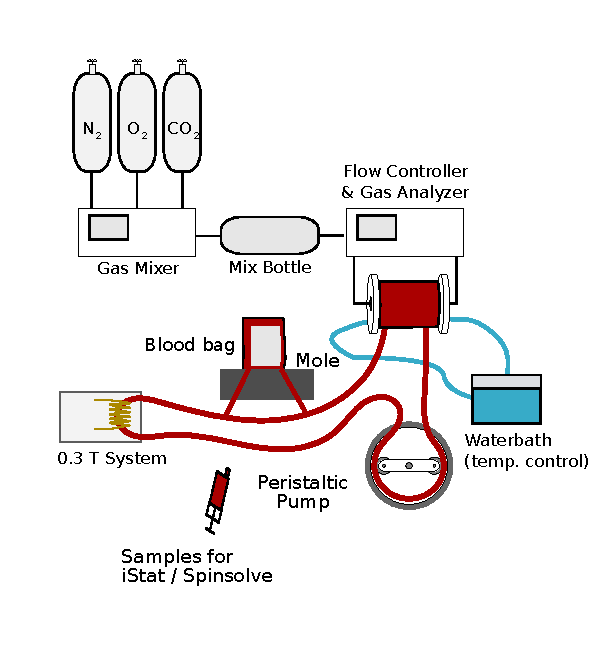
\includegraphics[width=0.8\textwidth]{figures/exptsetup/BloodMixingSetup.pdf}
\caption{Schematic of the Stopped flow setup}
\label{fig:exptsetup-stopflowschematic}
\end{figure}

A schematic of the flow stopped setup is shown in \autoref{fig:exptsetup-stopflowschematic}.
The main components are the roller pump and the oxygenation membrane, with the blood collection bag acting as a reservoir.
These are all joined by 1/4'' medical grade PVC tubing.
The total volume of this circuit was typically \SI{60}{\milli\litre}, with the blood bag containing 450 ml TODO check logbook.

The roller pump is used to generate flow around the circuit, by rotating the pump head to drive 2 rollers that squeeze the walls of the tube and force the blood along.
The pump is also designed for use in CPB surgery, and is a Stockert SIII, with a flow rate controllable from \SIrange{0.01}{6}{L/m} when used with the 1/4'' tube. TODOcheck?.
These versions of the flow circuit included a bypass section controlled by clamping the tubes so that the blood flow could be directed to around the reservoir, allowing for faster changes in the oxygenation due to a lower effective volume.
One important setting on the pump is the occlusion, which controls how much the tubing is squeezed as the pump head rotates.
Having the occlusion set too loosely causes the pump to become ineffective, as the blood can flow backwards through the pump, while setting it too tightly was found to cause damage to the red blood cells as they travel through the pump.
One problem with the model of pump used in these experiments does not have any sort of readout of the occlusion setting, so this had to be set at the correct value by following a testing procedure each time the occlusion was changed.

\subsection{Oxygenator and Gas Mixer}
A hollow-fibre membrane oxygenator was used to control the oxygenation of the blood in the circuit.
This was a Medtronic Affinity Pixie oxygenator, designed for use in paediatric CPB procedures.
It allows for gas exchange and temperature control of the blood flowing through, with the oxygenation controlled by the mix of gases going into the oxygenator.
This paediatric model was chosen to minimize the required priming volume, and it still provided more than enough capacity to oxygenate the blood at the flow rates used.
The temperature of the blood was regulated by flowing water from a temperature controlled waterbath through the oxygenator, which has a separate path built into it for this purpose.
The water bath temperature was set to \SI{35}{\degreeCelsius}, although this corresponded with a blood temperature at the outlet of \SI{33}{\degreeCelsius} at maximum flow rates (with lower temperatures at lower flow rates.)

The gas mix was set using a Dansensor MapMix 3 gas mixer, which allowed control of the different proportions of \Ntwo, \Otwo, and \COtwo flowing through the oxygenator.
The Oxygen fraction was typically varied from 0\% up to 21\%, the value of atmospheric air.
Nitrogen was used as a non-Oxygen containing gas, and between 2.5-5\% \COtwo was also added to ensure the pH of the blood sample remained stable over the course of the experiment (as these are linked by the bicarbonate buffer system in blood).
Gases for all experiments were used as supplied from BOC and were instrument grade or higher.
The output of the gas mixer flowed into a pressurised buffer tank before flowing into a Dansensor MapCheck Provectus gas analyser, which allowed us to check the fraction of the three gases which flowed into the oxygenation membrane.
This gas analyser also provided some flow regulation, although this was supplemented with an adjustable flow valve.
Typically, the gas flow rate was set to only \SIrange[per-mode=symbol]{1}{2}{\liter\per\minute} to avoid creating bubbles in the oxygenator.

\subsection{Blood collection}
Samples of whole blood were collected by venipuncture from healthy volunteers (taking place at Otago medical school).
This procedure was approved by the central health and disability ethics committee, and all volunteers provided written, informed consent.
Approximately \SI{450}{ml} of blood was collected into a blood bag containing \SI{66.5}{\milli\litre} CPD anticoagulant/preservative solution (Haemonetics Leukotrap WB system).
CPD solution is rated for storage of red blood cells for up to at least 3 weeks of storage\cite{Hessupdatesolutionsred2006}.
Blood samples were held at room temperature following collection, before undergoing leukoreduction filtering to remove white blood cells.
As it has been shown that the presence of white blood cells can adversely affect the condition of red blood cells in storage\cite{Hessupdatesolutionsred2006}.
Samples were then moved to a refrigerator and stored at \SI{4}{\degreeCelsius} until required for experiments (up to 30 TODO check! days for stopped flow experiments, up to 10 days for continuous flow experiments)

\subsection{NMR setup}
For these experiments, 3 different permanent magnet systems were used to obtain data at 3 different field strengths.
TODO pics of magnets!!

The first system was a 12 MHz (\SI{0.3}{T}) Halbach magnet array, with \SI{9}{cm} diameter bore and approximately \SI{20}{\centi\metre} long.
This magnet was repurposed from a previous experiment in the lab, and specifications are not available for it.
When combined with the home built coil and holder system described in \autoref{sec:exptsetup-coil}, the FID linewidth produced by the magnet was \SI{12}{\kilo\hertz}, which is relatively broad.

Because it uses permanent magnets, it requires a stable temperature in order to have a stable field.
This was set up using a temperature controlled water bath, which pumped wat at a constant \SI{30}{\celsius} through tubes wrapped around the magnet.
On top of this, the magnet was wrapped in a layer of foam, and a layer of mylar sheeting to insulate it from the room.
To decrease the effect of electrical noise on the measurements, the magnet assembly was also surrounded by a thin coppper mesh blanket.

The second magnet system used was the NMR MOLE, previously developed by Manz et al\cite{ManzmobileonesidedNMR2006}.
The NMR MOLE operates at a field of \SI{0.1}{T} and is a single sided device, which produces a `sweet spot' in the region above the magnet.
The sweet spot is where the combination of magnetic field and RF produced by the coil on the surface are able to create resonance, which defines where signal comes from.
In this case, the sweet spot was a pair of regions marking out a \SI{3}{cm} circle over the RF coil (TODO see figure? honours project).
While earlier experiments attempted to position the tube containing blood over the sweet spot, in later experiments, it was decided that it was simpler and more reliable to place the blood bag on the top of the MOLE.
As with the Halbach array, the MOLE is also sensitive to temperature, so an electronic temperature controller and wire heater were used to keep it stable at \SI{29}{\celsius}.

The design of the magnet array in the MOLE creates strong magnetic field gradients across the sweet spot.
This creates a wide range of resonance frequencies, and means that it was not possible to measure an FID from the system.
It was also found that this limited the possible range of CPMG echo times, as echo times longer than \SI{1}{ms} were caused excessive signal attenuation.
This limited experiments with this system to short echo times.

The third magnet system used was a Magritek Spinsolve, which is another permanent magnet based NMR system operating at \SI{1}{T}.
The Spinsolve is designed for chemical spectroscopy, so has a very homogeneous field, and can produce a linewidth of less than \SI{0.1}{Hz}.
It also uses standard 5 mm NMR sample tubes, so it could not be used inline in the flow circuit like the other two systems.
Because of this, experiments on the Spinsolve required withdrawing a small amount of blood and transferring it into an NMR tube.
This meant that that there were typically delays between removing the blood from the circuit and taking measurements on it, which may cause changes in the state of the blood.

Both the Halbach and MOLE systems were controlled on computers running Magritek Prospa, and used Magritek Kea 2 spectrometers to run the NMR experiments.
The Spinsolve was also controlled from a computer with a newer version of Prospa.
CPMG experiments were run using the default CPMG macros included in Prospa, with batch scripts set up to automate taking measurements at multiple echo times.

\section{Continuous flow setup}
\label{sec:exptsetup-contflow}

To be able to get better data on how \Ttwo is affected by \SOtwo at different fields, we decided to move to a continuous flow method, where the \SOtwo was slowly ramped from low to high oxygenation, while the \Ttwo was constantly measured.
This required a number of changes to the stopped flow setup, including the use of the baby-MRI magnet, and the development of a system for continuours \SOtwo tracking.


\begin{itemize}
\item Flow Circuit changes
\item different magnet
\item sO2 measurement - optical sensor, calibration
\item Flow stability
\end{itemize}

\subsection{Flow Circuit Changes}

\subsection{Coil Assemblies and Electronics}
\label{sec:exptsetup-coil}
A new coil holder, coil assembly and tuning and matching circuit was designed to fit into the baby-MRI system and also used in the Halbach magnet array experiments in  \autoref{ch:stoppedflow}.
It was designed with exchangeable coils and tuning and matching capacitors so that the probe could be used at multiple fields / frequencies.
It consists of a probe (outer piece), which holds the coil assembly and the tuning and matching circuit inside the bore of the magnet (which had the same diameter in the two magnets).

The coils are \SI{2}{cm} long, and have a diameter of \SI{1}{cm}, so that the 1/4'' tube can be passed through the coil,
Different numbers of turns were used for the three different coils, to be able to use the coils at different frequencies (More turns causes more inductance, and a lower resonant frequency.)
In the initial design of the coil assembly, the coil was constructed from \SI{0.67}{mm} Copper wire wrapped around a rolled up acetate cylinder.
A second version of the coil assemblies used 3D printed forms made from ABS plastic (to decrease unwanted signal), with the same wire and number of turns.

TODO:picture of the coils
TODO:picture of the T\&M circuit

The tuning and matching circuit was also designed and manufactured for this probe.
It allows for the capacitors to be exchanged, using small PCBs with different capacitors attached.
While high frequencies
The different capacitors allowed the probe to be tuned and matched at frequencies ranging from \SIrange{2}{60}{\mega\hertz}.
As the probe is located inside the magnet, the capacitors are all of a non-magnetic type (AVX Hi-Q or Cornell Dubilier CDE MCM series) and are rated for high voltage (\textgreater\SI{500}{V}.)
The tuning and matching circuit also contains variable capacitors which are used for fine tuning the match frequency.

S\textsubscript{11} simulations were run in Qucs Spice to find the best values of C\textsubscript{T} and C\textsubscript{M} at a range of frequencies.

\chapter{Stopped flow \SOtwo measurements}\label{ch:stoppedflow}

As a first step in this research, experiments on blood using a stopped flow setup were completed, using a similar protocol and design used in previous work by the group.
Stopped flow measurements are the typical method used in the literature for these blood oxygenation \Ttwo experiments, and there a number of examples in the literature\cite{BrooksComparisont2relaxation1995,BryantMagneticrelaxationblood1990,GomoriNMRRelaxationTimes1987} (although as mentioned in the introduction, relatively few at low field.
These experiments used the stopped flow experimental setup from \autoref{ch:exptsetup}, with 3 different magnet systems at different fields to observe changes in \Ttwo at a number of levels of oxygenation.
These also provide a benchmark for the continuous flow setup, as it removes any effects which occur because of flow.

\section{Experimental Protocol}
For this series of experiments, measurements of \Ttwo were made at a series of oxygenation steps, which we attempted to set by adjusting the gas mix going into the oxygenator.
These steps are shown graphically in \autoref{fig:sf-protocol}
After the flow circuit was assembled, the blood sample was loaded into the tubes and oxygenator, using the standard connectors on the bag.
The pump was switched on, and gas at 21\% \Otwo was flowed through to bring the oxygenation and temperature of the blood up to the 100\% starting point for the experiments.
The blood was allowed to flow through the circuit for the temperature to stabilise, before an initial test with the iStat.
During this time, the probes were tuned and matched, and pulse sequence parameters such as pulse power and \textit{B\textsubscript{1}} frequency were calibrated (using FIDs on the Halbach system, and CPMG detection on the MOLE.)
\begin{figure}[t]
\centering
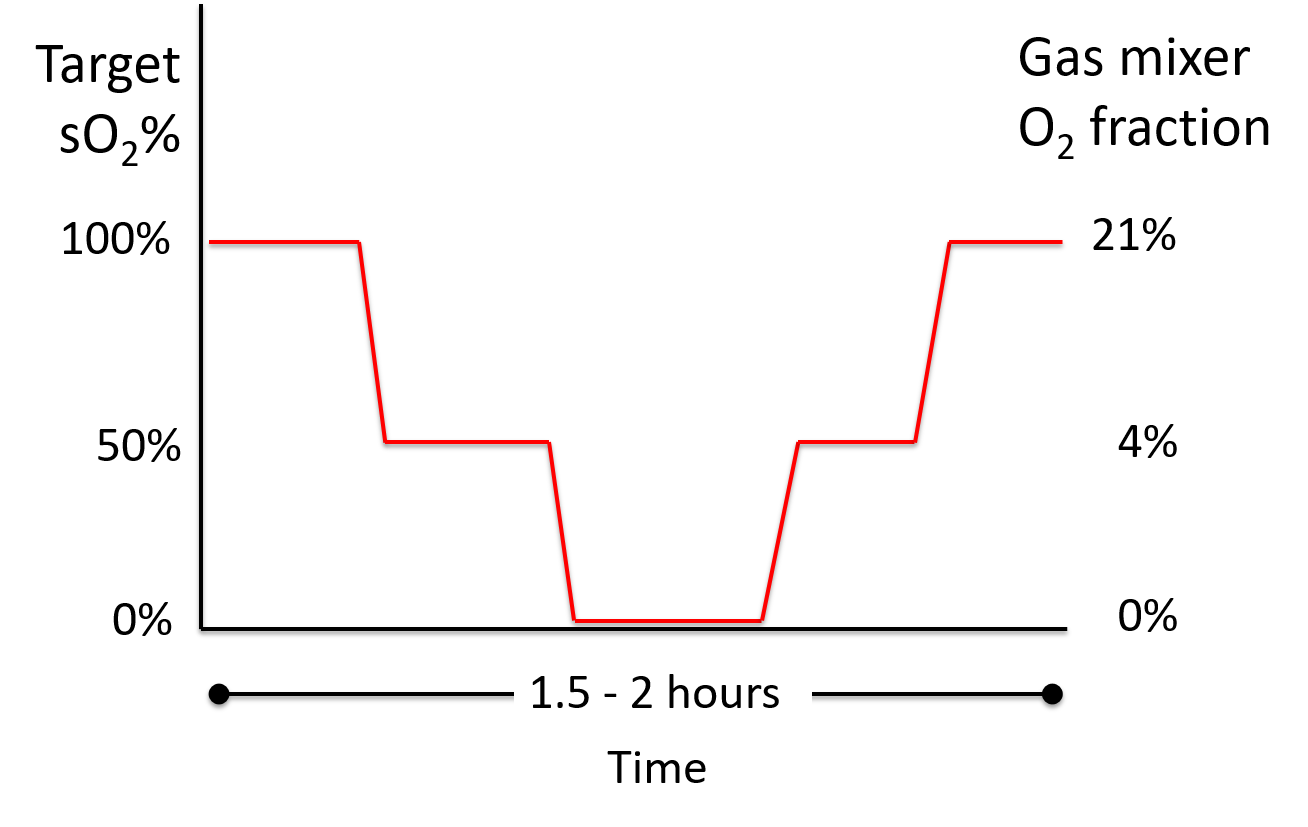
\includegraphics[width=0.7\textwidth]{figures/stoppedflow/stoppedflowprotocol.png}
\caption{Outline of experimental protocol for stopped flow experiments}
\label{fig:sf-protocol}
\end{figure}

If this showed that the pH, \SOtwo and HcT were normal, the flow was stopped and measurements on the two in-line NMR systems were started.
It was possible to adjust the pH of the blood through the addition of sodium bicarbonate solution.
Typically \TR = \SI{1.5}{s}, with echo times of \SIlist{0.25;0.5;1;5}{ms} on the Halbach, and \SIlist{0.25; 0.5; 1}{ms} on the MOLE (these were limited by the magnetic field gradients in each system).
The number of echoes was adjusted to create an echo train \SI{600}{ms} long.
4 scans with phase cycling were used on the Halbach, but the poorer signal to noise on the MOLE meant that 16 scans were required.
Once these measurements had completed, the pump was turned on briefly to agitate the blood and minimize any effects of settling before repeating the NMR measurements.
A \SI{2}{ml} sample of blood in the circuit was also taken out and syringed into a clean \SI{5}{mm} NMR tube for the Spinsolve measurements.
These tubes were sealed with the caps provided by the manufacturer.
On the Spinsolve, typical experimental parameters were \TR = \SI{20}{s} with a 4 scan phase cycle, and with 4 echo times: \SIlist{0.5;2.5;5;10}{ms}.
Again, the number of echoes was set to give an echo train with a fixed length of \SI{10}{s}.

\begin{figure}[t]
\centering
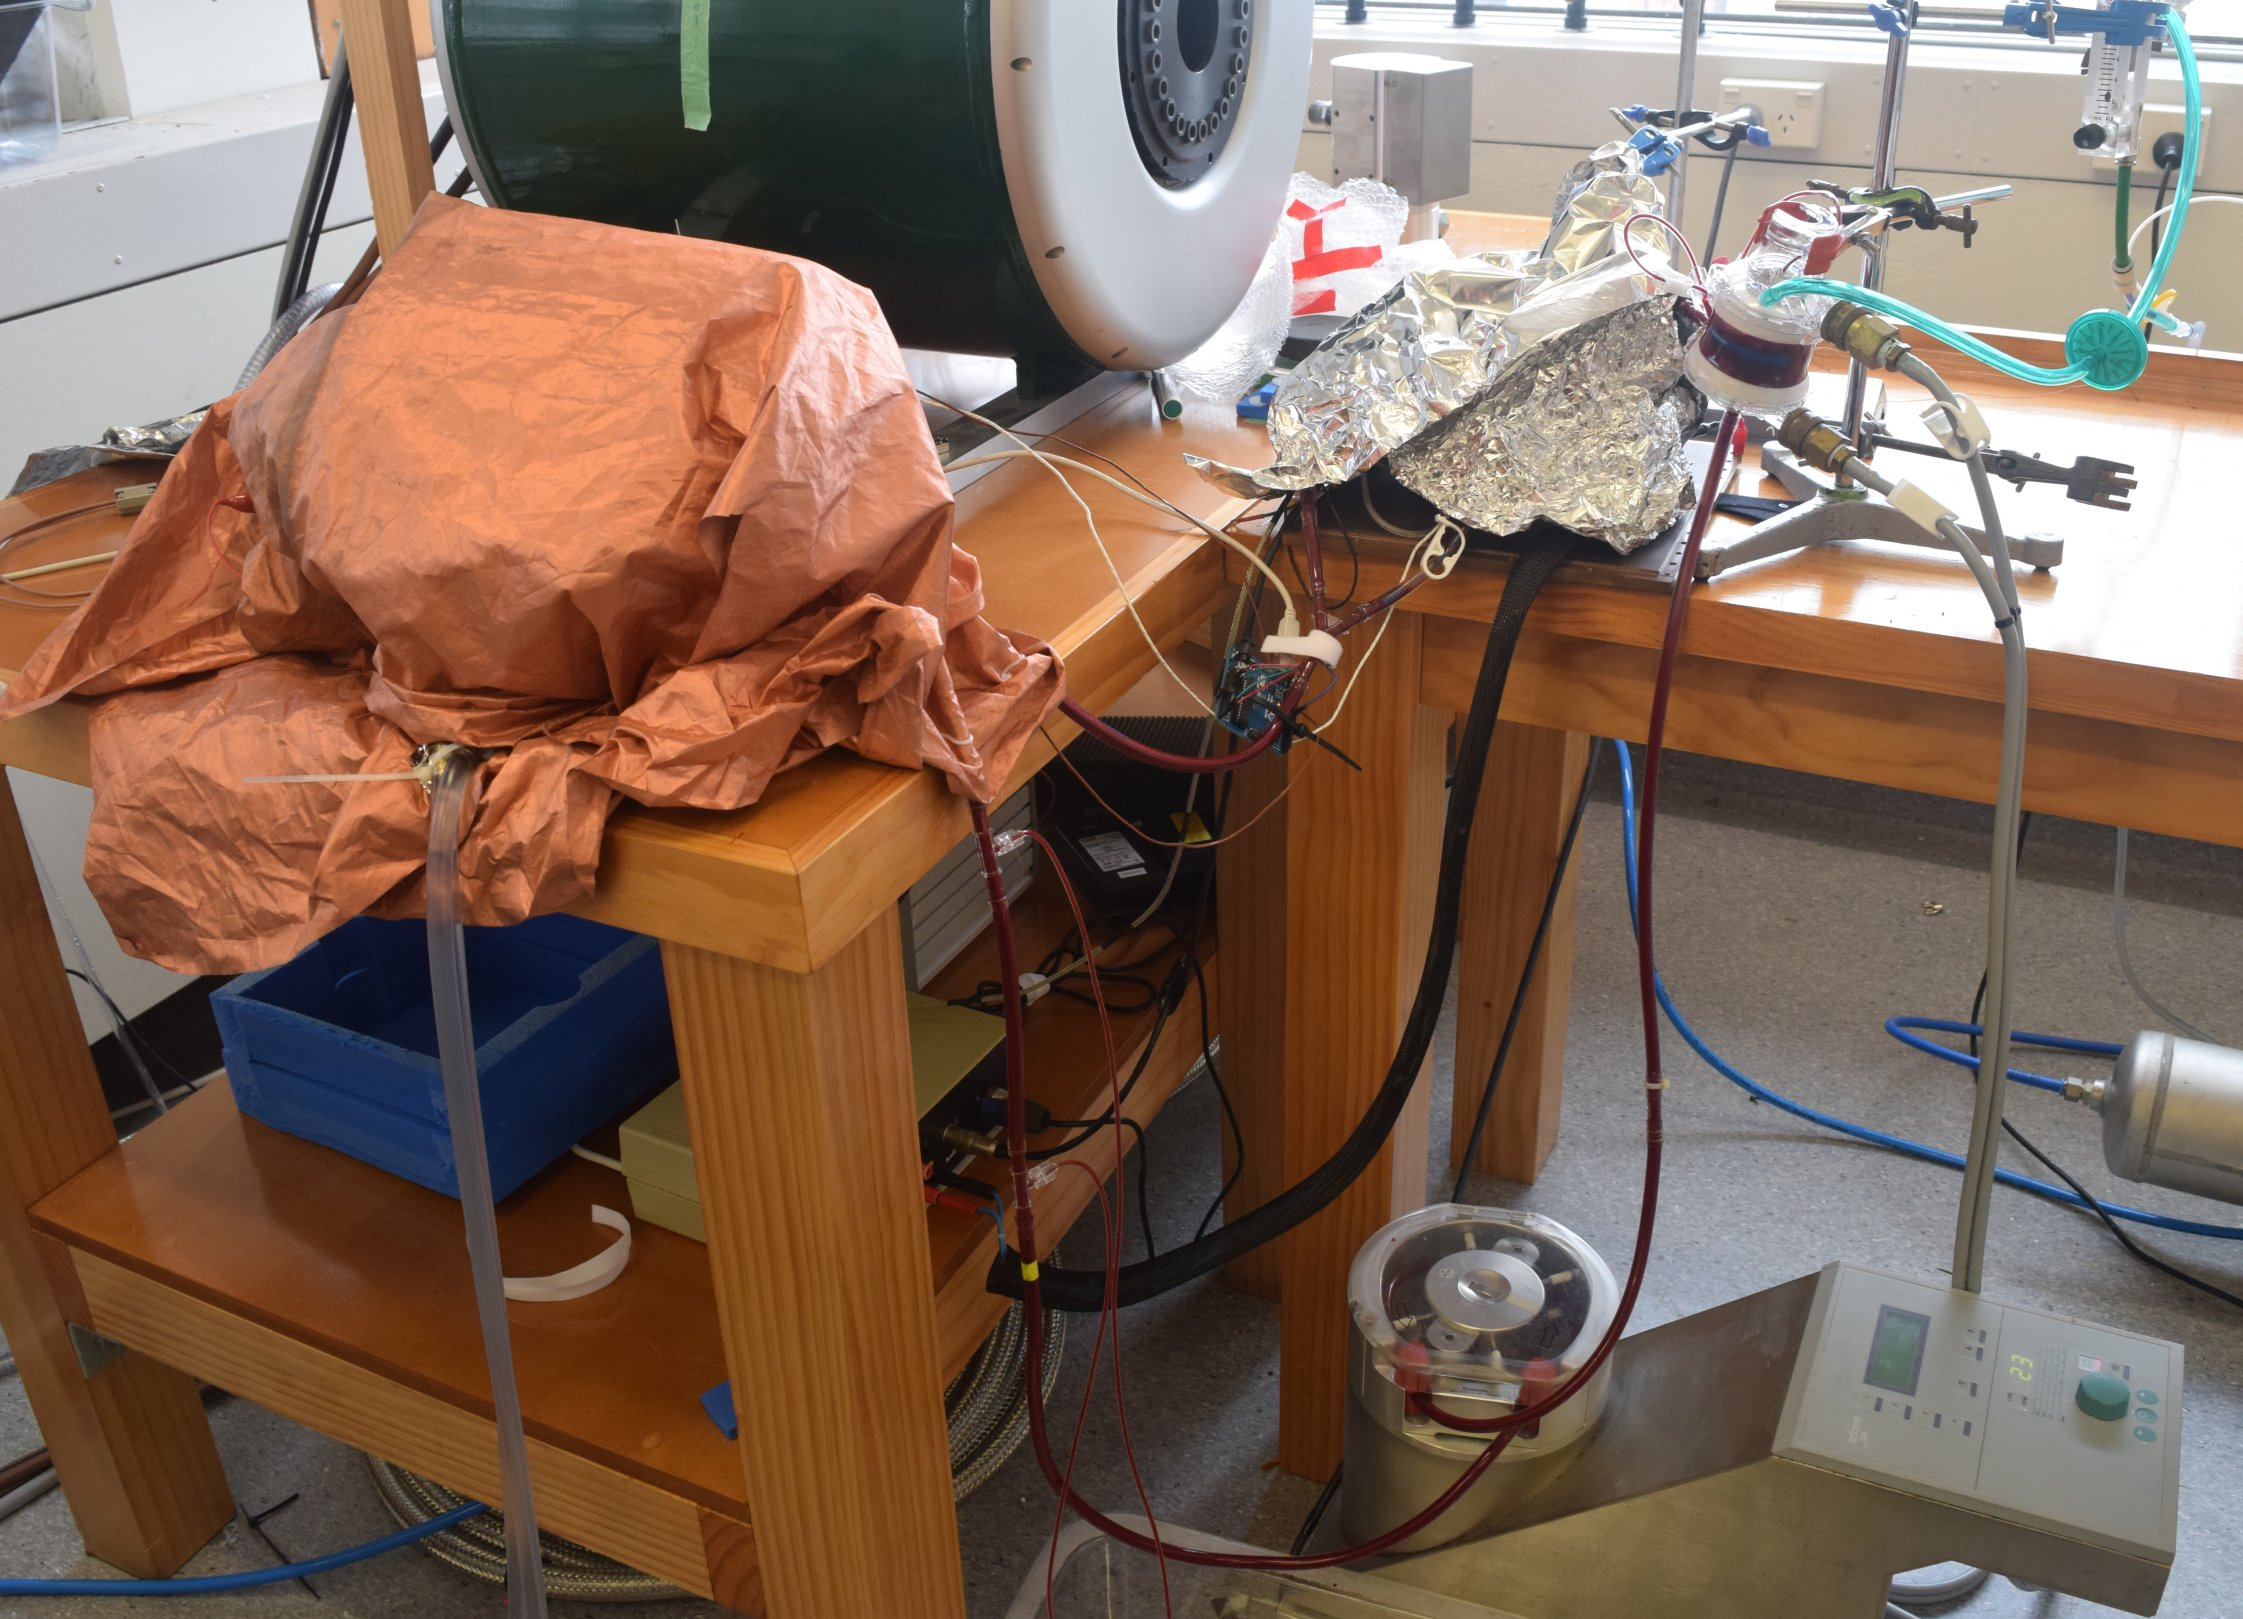
\includegraphics[width=0.8\textwidth]{figures/stoppedflow/stoppedflowsetup.jpg}
\caption{Experimental setup for stopped flow experiments (gas mixer and analyser not shown)}
\label{fig:sf-stoppedflowsetup}
\end{figure}

The \SOtwo was then lowered to an intermediate value (around 50\%).
Flow was turned back on and the gas mix set to 5\% \Otwo, which we had found produced these levels of oxygenation.
After waiting for the \SOtwo to reach the desired level, a sample of blood was taken from the flow circuit and the iStat was used to confirm the \SOtwo.
The flow was stopped, and two sets of NMR measurements were completed as above, with samples also removed for the Spinsolve.

This process was repeated again to measure \Ttwo at a very low oxygenation (10\% or less), by setting the gas mix to 0\% \Otwo.
Afterwards, these steps were reversed to increase the oxygenation again, taking a measurement at an intermediate value of \SOtwo on the way up as well.

Data was extracted and processed using Python, in JuPyter notebooks.
Each echo train is phased, and each echo is summed to give a single value for the signal at each echo time.
The resulting decay is fit to a monoexponential decay using non-linear least squares fitting, which results in a single \Ttwo value at each \SOtwo.

\section{Results}
\subsection{Spinsolve results}
Two examples of the CPMG decays measured on the Spinsolve are shown in \autoref{fig:sf-spinsolveCPMG}.
Plotting the log of the echo amplitudes against time gives a straight line, which indicates that the decay is mono-exponential.
This agrees with what is reported in the literature.

This data also shows even-echo rephasing occuring in the decays measured with long echo times (in red).
Where this was visible, only the even echoes were used in the curve fitting routine to find \Ttwo.

%Graph generated in processBloodOxygenation1/Spinsolve data 170728
\begin{figure}[ht]
\centering

\begin{subfigure}[t]{0.48\textwidth}
\caption{\SOtwo = 95\%}
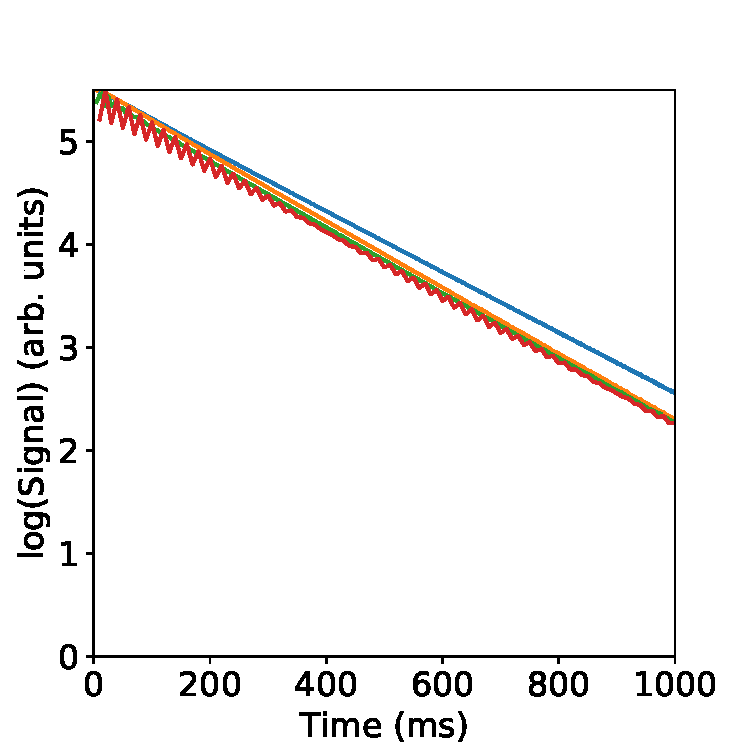
\includegraphics[width=\textwidth]{figures/stoppedflow/spinsolveCPMG95.pdf}
\end{subfigure}
\begin{subfigure}[t]{0.48\textwidth}
\caption{\SOtwo = 9\%}
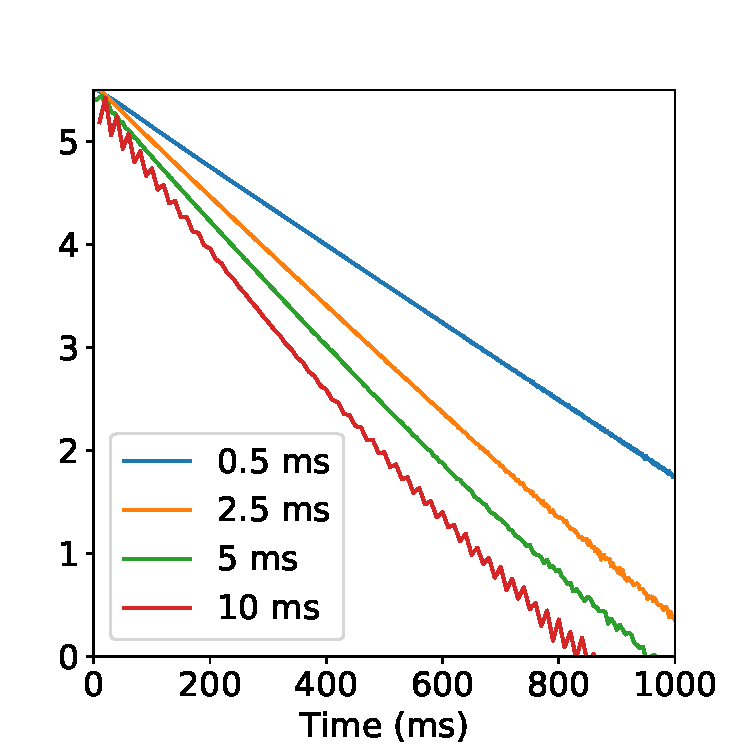
\includegraphics[width=\textwidth]{figures/stoppedflow/spinsolveCPMG9.pdf}
\end{subfigure}

\caption{Examples of CPMG decays measured on the Spinsolve for oxygenated and deoxygenated blood}
\label{fig:sf-spinsolveCPMG}
\end{figure}

Decays were measured at a range of oxygenations and fitted to obtain \Ttwo.
These results are shown in \autoref{fig:sf-spinsolveT2SO2}.

%Graph generated in processBloodOxygenation1/Spinsolve data 170728
\begin{figure}[ht]
\centering
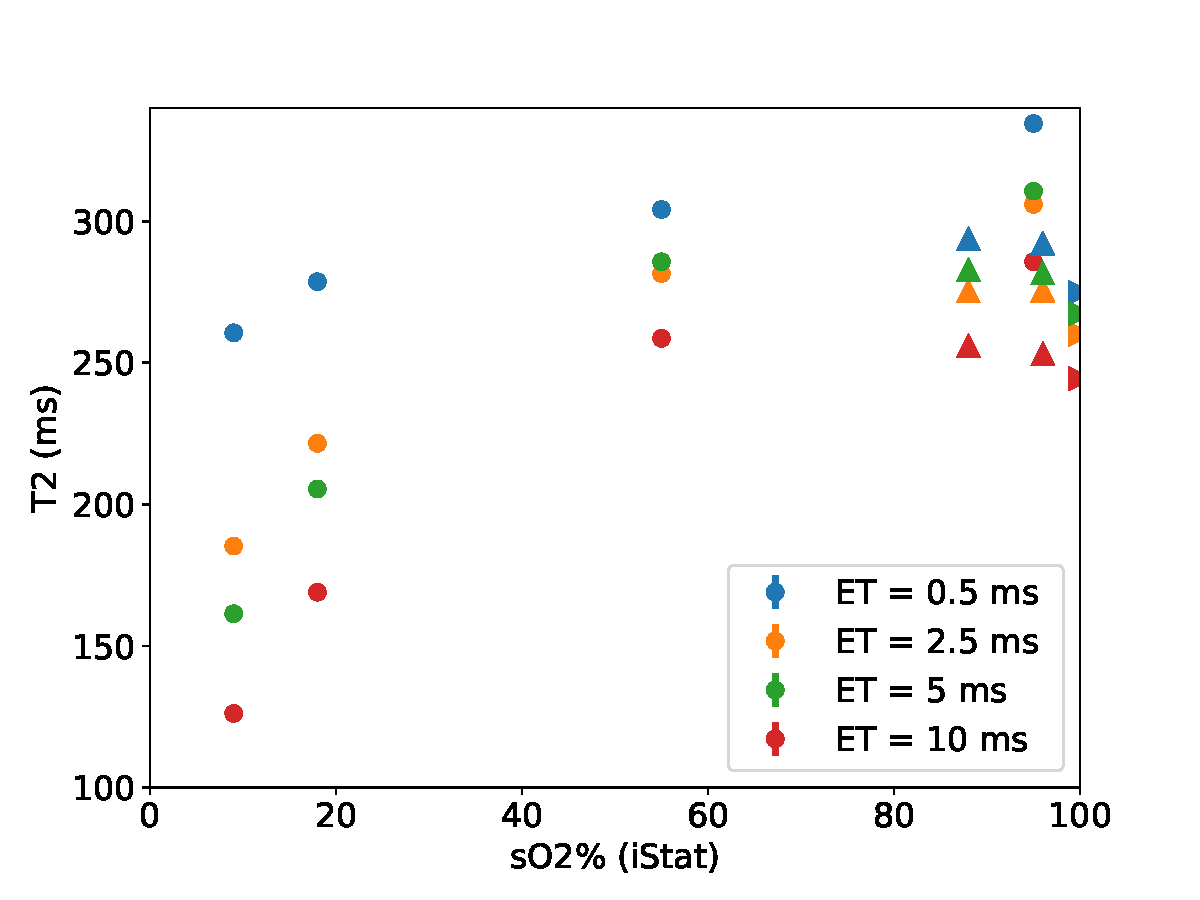
\includegraphics[width=\textwidth]{figures/stoppedflow/spinsolveT2SO2down.pdf}
\caption[\Ttwo vs. \SOtwo measured on the Spinsolve]{\Ttwo at different levels of oxygenation, measured on the Spinsolve. Circles indicate samples measured when deoxygenating the blood, while upwards pointing triangles are samples when oxygenating it (see experimental protocol). Right pointing triangles are a sample hyperoxygenated with 30\% \Otwo}
\label{fig:sf-spinsolveT2SO2}
\end{figure}

As the oxygenation of the blood was lowered, the \Ttwo decreases from \SI{334}{ms} to \SI{260}{ms} at the short echo time, while changes more drastically from \SI{285}{ms} to \SI{126}{ms} at the longest echo time.
This shows that the changes in oxygenation are visible in this \SI{1}{T} system.
The shorter \Ttwo at long echo time is expected, as there is more time for dephasing to occur, as discussed in TODO backgroundsection!!.
The separation between the short echo time and long echo time \Ttwo{}s also increases at lower \SOtwo.
This is predicted by theory, as the susceptibility difference and induced field inhomogeneity is increased with high levels of deoxyhaemoglobin.

One difficulty we had was recovering the original \Ttwo value when the blood was re-oxygenated.
This is shown by the two samples measured while oxygenating (triangles in \autoref{fig:sf-spinsolveT2SO2}.
A number of experiments were conducted to investigate the cause of this, and these are discussed below.

\subsection{Halbach results}
%Graph produced in Halbach 170726
\begin{figure}[h]
\centering
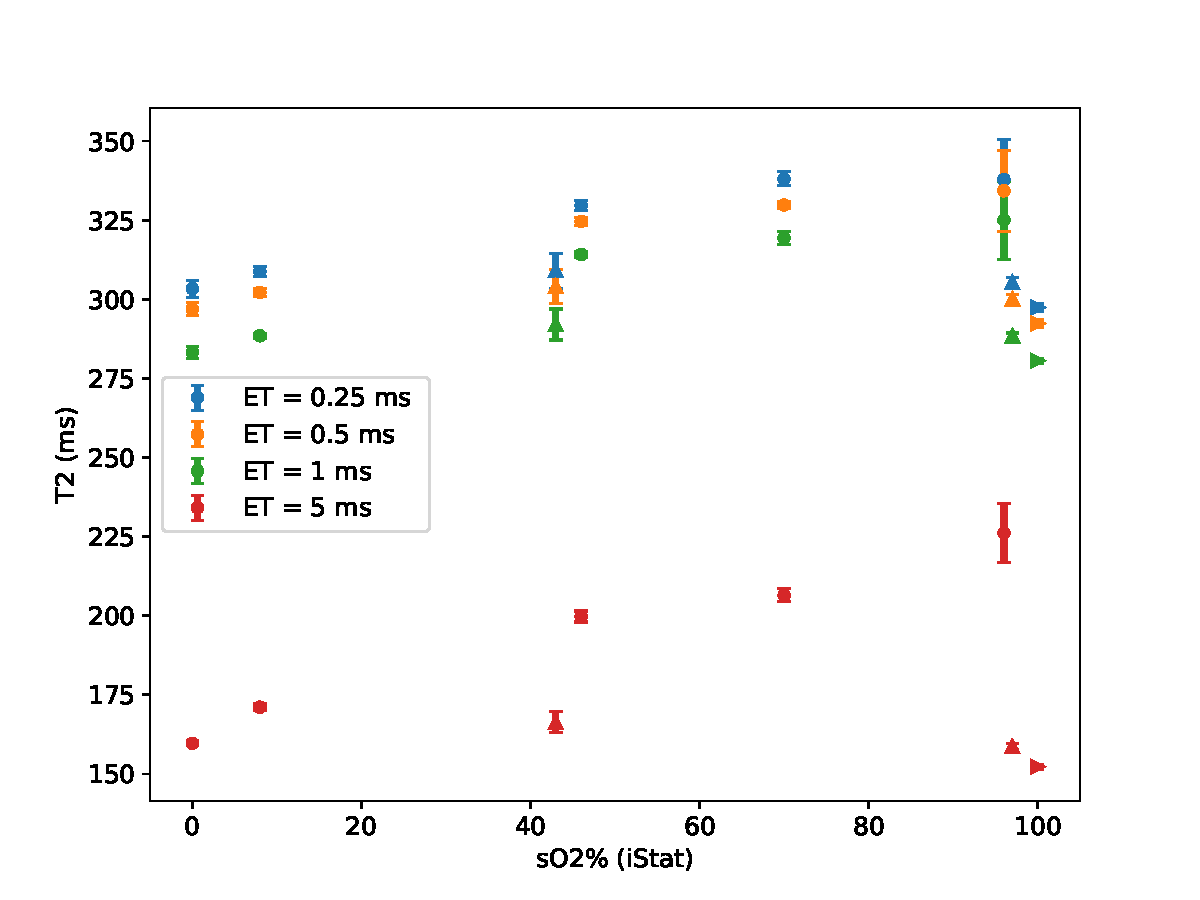
\includegraphics[width=\textwidth]{figures/stoppedflow/halbachT2SO2.pdf}
\caption[Stopped flow \Ttwo vs. \SOtwo measured on the Halbach system]{\Ttwo vs. \SOtwo measured on the Halbach system. Circles indicate samples measured when deoxygenating, upwards triangles are measured when oxygenating and right-pointing triangles are a sample oxygenated with 30\% \Otwo. Error bars represent standard error (n=3)}
\label{fig:sf-halbachT2SO2}
\end{figure}

The Halbach magnet system was run inline with the flow circuit, making it easier to measure more data points.
As with the Spinsolve results, the CPMG decays were found to be monoexponential, however there was no appearance of even echo rephasing in the CPMG decays.
In this experiment, the deoxygenation causes the \Ttwo to decrease from \SI{337}{ms} to \SI{303}{ms} fot the short echo time, and from \SI{226}{ms} to \SI{152}{ms} for the \SI{5}{ms} echo time.
The strong field gradients in this system means that the CPMG experiments are sensitive to the diffusion of protons moving through the gradient, which causes longer echo times to measure a shorter \Ttwo.
This can be seen in the position of the \SI{5}{ms} points (red), which are significantly lower than points at \SI{<1}{ms}.
In this experiment, measurements were also completed with echo times of \SIlist{8;12}{ms}, but these did not show any trends due to the strong relaxation from the field inhomogeneities.

Like in the Spinsolve experiments, the \Ttwo values in this experiment did not return to the same levels they did at the start of the experiment after reoxygenating, which suggests that this change is not solely related to the sampling method and storage of the Spinsolve samples.
The decrease from the initial \Ttwo measurement to the reoxygenated measurement appears to be approximately the same size (\SI{40}{ms}), although the decrease at the \SI{5}{ms} echo time is much greater.
This may also be related to problems with the Halbach magnet and probe, for example, changes in magnet temperature over the experiment time or slight movements or rotations of the probe inside the magnet, which would alter the gradients seen be the sample.

\subsection{MOLE results}
%Graph from Mole 170728
\begin{figure}[h]
\centering
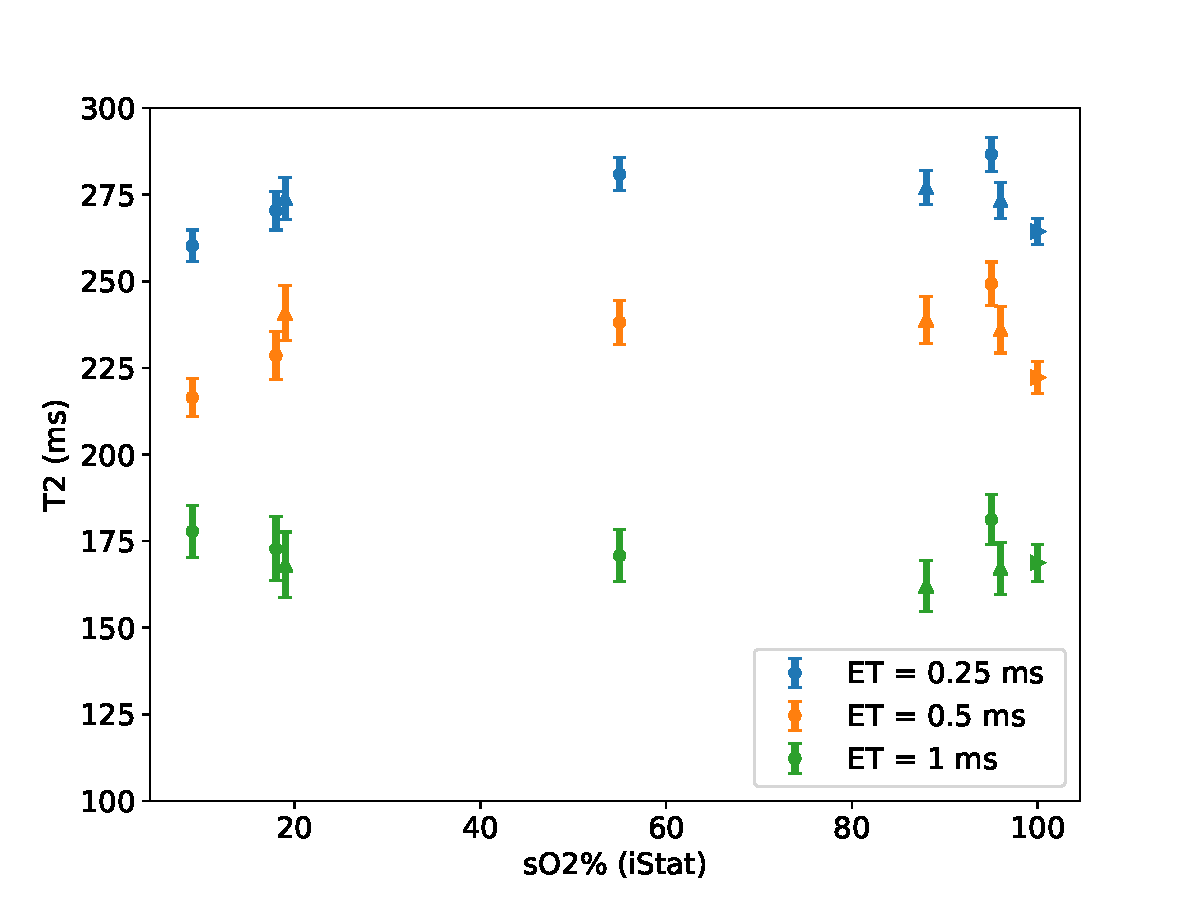
\includegraphics[width=\textwidth]{figures/stoppedflow/moleT2SO2.pdf}
\caption[Stopped flow \Ttwo vs. \SOtwo measured on the MOLE system]{\Ttwo vs. \SOtwo measured on the MOLE system. Circles indicate samples measured when deoxygenating, upwards triangles are measured when oxygenating and right-pointing triangles are a sample oxygenated with 30\% \Otwo. Error bars represent standard error (n=3)}
\label{fig:sf-moleT2SO2}
\end{figure}
%
Measurements on the MOLE had a significantly lower signal to noise than the other two systems.
This is related to both the reduced field strength (\SI{0.1}{T}), and the single-sided design of the magnet system.
Because of this, measurements took longer to acquire than on the other systems and the largest source of experimental uncertainty was from noise in the fitting process.

As expected, the change in \Ttwo as oxygenation was decreased was smaller again than in the higher field Spinsolve and Halbach system measurements.
At the \SI{0.25}{ms} echo time, the decrease from oxygenated to deoxygenated is \SI{25}{ms}, but at the \SI{1}{ns} echo time, the decrease is only \SI{5}{ms} (which is within experimental uncertainty.)
Additionally, the field inhomogeneity of the MOLE means that there is a significant decrease in the measured \Ttwo due to diffusion through the gradients of the magnet system.
Along with the decrease in the stregnth of the effect at this field, this could explain why there is little to no change at the \SI{1}{ms} echo time.

These results also show that \Ttwo is lower after reoxygenating, with a decrease of approximately \SI{15}{ms} between the initial \Ttwo and the \Ttwo after reoxygenation.
It is unlikely to be due to changes in the magnetic field gradients as the MOLE temperature is very well controlled, and the sample was the entire blood bag, which is larger than the sweet spot of the magnet.

\subsection{Field comparison}
Results for the different fields are combined in \autoref{fig:sf-fieldcomparison}, after converting the \Ttwo values for oxygenated and deoxygeneated blood into \Rtwo.
Although the data from the MOLE is strongly affected by its inhomogeneous field, taking the difference of the oxygenated and deoxygenated \Rtwo{}s should cancel this effect.

%Graph from Spinsolve 170728
\begin{figure}[h]
\centering
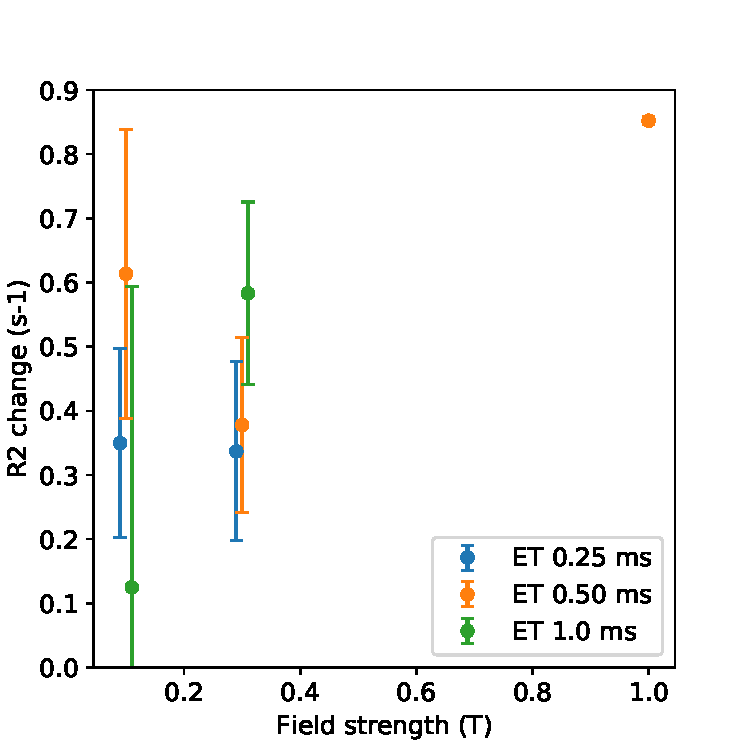
\includegraphics[width=0.8\textwidth]{figures/stoppedflow/fieldcomparison.pdf}
\caption[Change in \Rtwo for the three stopped flow systems]{Change in \Rtwo for the three stopped flow systems. Data points show \Rtwo\textsubscript{\textit{deoxy}} -- \Rtwo\textsubscript{\textit{oxy}} to remove the effect of background gradients. Note points are moved on the x-axis to allow comparison}
\label{fig:sf-fieldcomparison}
\end{figure}

\autoref{fig:sf-fieldcomparison} shows that the \Ttwo decrease is much larger at \SI{1}{T}, although data was only collected at the \SI{0.5}{ms}.
Additionally, the \SI{0.1}{\tesla} measurement shows that the change in \Rtwo is higher or the same as than the data point at \SI{0.3}{T}, which does not agree with the quadratic dependence from theory, however, the uncertainty in the MOLE data points is much larger.

%It is also possible that the exchange/diffusion theory is not as effective at these short echo times, and other processes are occuring, this might be discussed below TODO!!!!

\section{Discussions}

These results confirm that \Ttwo when decreasing \SOtwo occur at low fields, in agreement with the literature.
As noted in the introduction however, there are relatively few examples in the literature to compare them to.
Brooks et al. studied the field dependence of the \Ttwo decrease for oxygenated and deoxygenated blood, and found that the size of the \Rtwo change scales with \Bzero  squared\cite[Fig.1]{BrooksComparisont2relaxation1995}.
For their study however, they used a more conventional \SI{4}{ms} echo time, which makes the \Rtwo change from oxygenated to deoxygenated much larger (on the order of \SI{4}{s^{-1}} at \SI{0.5}{T}.)
This means that their results are not directly comparable with the results in \autoref{fig:sf-fieldcomparison}, where the echo time is less than \SI{1}{ms}.

%While applying the exchange model discussed in TODO(the background) directly to these results is not possible due to the effect of the field gradient, these gradient effects can be subtracted to give an estimate of the increase in \Rtwo due to the \SOtwo change.
%This leaves the value for \Rtwo due to only the deoxygenation, which should be equivalent to the exchange term in the chemical exchange model (\autoref{eq:LMsimp}).
%The results in \autoref{fig:sf-fieldcomparison} do not agree with the model, as the model relies on the approximation that the exchange or diffusion rate is much faster than the CPMG refocusing rate.
%Further investigation is needed to be able to determine the mechanism causing the change in \Ttwo at short echo times, and how sensitive it is to changes in \SOtwo.
%This may be particularly important for application in single sided devices, which typically use short echo times.

We also encountered trouble with recovering the intial \Ttwo when reoxygenating the blood.
This was visible in all results above, where at high \SOtwo{}s, the reoxygenated \Ttwo values (upwards triangles)  are typically lower than the initial values (circles) by \SIrange{10}{40}{ms}.
In this set of experiments, several hypotheses were tested to investigate the cause of this.
The fact that it occured across all three systems (including the Spinsolve, which was used not part of the circuit) suggests that it is due to a physical change in the blood and not only related to changes in the flow circuit (although movement of the Halbach probe could not be ruled out.)

One possibility was that the blood was not completely reoxygenated, which could occur if the blood was damaged during storage or or the time at extremely low \SOtwo, and caused the \SOtwo measurement on the iStat to be inaccurate.
To test this, samples were hyper-oxygenated with 30\% \Otwo (rather than 21\%).
This caused an increase in the p\Otwo from \SIrange{110}{150}{mmHg} in the normally reoxygenated blood to \SIrange{180}{200}{mmHg} in the hyperoxygenated blood, and should have caused more of the remaining deoxy-haemoglobin to become oxy-haemoglobin, raising the \Ttwo.
Interestingly, we observed a further decrease in \Ttwo in all cases, shown by the right-triangles in the results.
This is not likely to be due to the paramagnetic effect of dissolved Oxygen, as this should have an extremely small effect on the \Ttwo at these relatively low p\Otwo values.
Ma et al. found that dissolved Oxygen in blood plasma causes \Rtwo to increase by \SI{2.3e-4}{s^{-1}\per\mmHg}~\cite{Maeffectdissolvedoxygen2016}, which would correspond to a change of \SI{0.04}{s^{-1}} at \SI{200}{mmHg}.

Another possibility was that a property of the blood had changed in the circuit, with some parameter that affects \Ttwo being different, for example the haematocrit increasing due to separation of plasma and red blood cells in the blood bag.
However, testing with the iStat (TODO probably!) showed no significant changes in the initial and final parameters.
TODO check iStat pH change, HcT change, K+ conc., HcT

Instead, we investigated whether red blood cells were being damaged by flowing through the circuit, and that this damage caused a decrease in \Ttwo.
This would explain the \Ttwo decrease after hyperoxygenation, which would be caused by spending more time in the flow circuit.
To test this, samples of the blood were removed from the circuit before and after the experiment.
These were centrifuged to separate the red blood cells and plasma, and the colour of the plasma was compared to identify whether significant haemolysis had occured.
An example of one test is included in \autoref{fig:sf-bloodbeforeafter}.
This effect was studied more quantitatively when it occured in the continuous flow experiments described in \autoref{ch:cont}.

\begin{figure}[t]
\centering
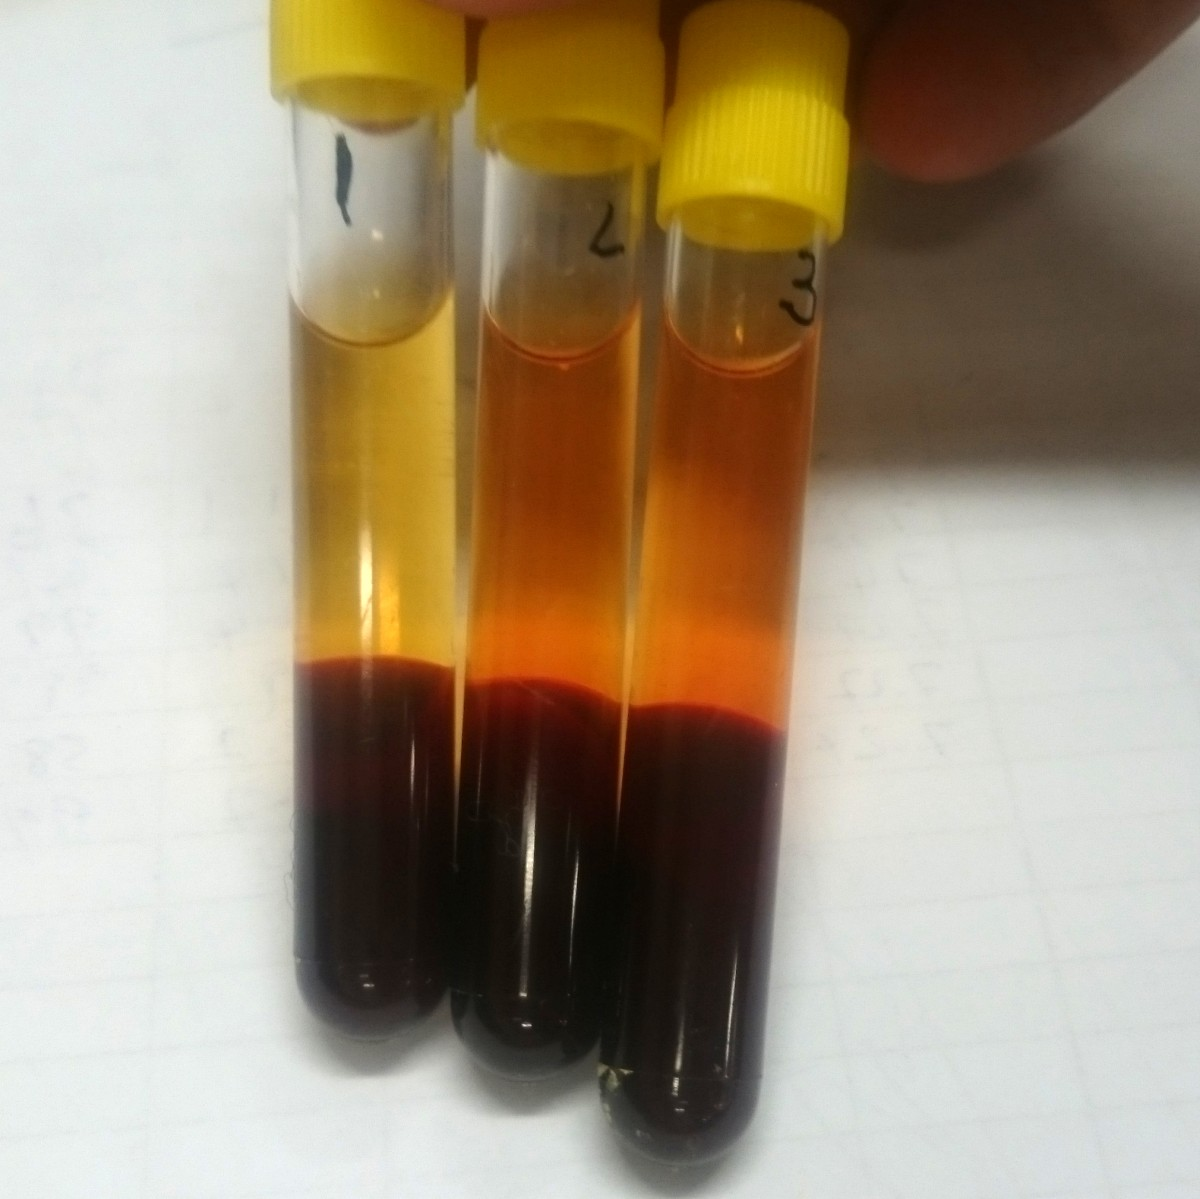
\includegraphics[width=0.5\textwidth]{figures/stoppedflow/samplecheck.jpg}
\caption[Centrifuged blood samples from start and end of experiment]{Centrifuged blood samples from before (tube 1, left), during (tube 2), and after stopped flow experiments (tube 3, right). Note the redder colour from the tubes on the right}
\label{fig:sf-bloodbeforeafter}
\end{figure}

While these results confirm that changes in \SOtwo can be observed at low field, there were some difficulties with this method of collecting data.
As the stopped flow system requires the flow to be stopped, it is possible that the blood could be changing within the scan time due to factors such as temperature dropping, or red blood cells separating from the plasma.
It was also very difficult to be able to `hit' desired intermediate values of oxygenation.
This is because of haemoglobin's strong affinity for Oxygen, which creates the very steep curve discussed in TODO(\SOtwo p\Otwo curve in background).
To be able to reach a specific intermediate levels of oxygenation would require more precision and stability in the gas mix output than were possible with this experimental setup.
Therefore, the continuous flow setup discussed in \autoref{sec:exptsetup-contflow} was designed for the next set of experiments.
Because the introduction of flow complicates everything, these stopped flow results are used as a benchmark for the continuous flow experiments.

%\chapter{Devlopment of a method for continuous \SOtwo measurement}
\label{ch:contsetup}

This chapter is about the system developed to continuously measure the \Ttwo of blood flowing in the circuit as the \SOtwo changes
\section{Experimental methods}

\chapter{Continuous \SOtwo measurement}
\label{ch:cont}

This chapter is about all the results from the continuous loop setup

\chapter{Models for \Ttwo relaxation enhancement}\label{ch:models}

As discussed in Chapter \ref{ch:background}, researchers have developed a number of models to explain the decrease in \Ttwo of the water protons in blood.
Thulborn originally applied the Luz-Meiboom equation to describe the decrease in \Ttwo and its dependence on the CPMG echo time\cite{ThulbornOxygenationdependencetransverse1982}.
Another model has been proposed by Jensen and Chandra, which more describes the dephasing of water protons that diffuse through areas of magnetic field inhomogeneities \cite{JensenNMRrelaxationtissues2000}.
Generally, the two models predict the same behaviour at short echo times \SIrange{1}{3}{ms} and at long echo times (\SI{>20}{ms})\cite{BrooksT2shorteningweaklymagnetized2001}, but in the intemediate range, the two models give different values for the magnitude of the \Ttwo change.
Additionally, experiments comparing the two models have found that at clinical MRI fields (1.5 T and up), both models provide good agreement with experimental data \cite{StefanovicHumanwholebloodrelaxometry2004,ChenHumanwholeblood2009,GardenerDependencebloodR22010,GrgacHematocritoxygenationdependence2013}.
Because of this, the Luz-Meiboom equation is typically used when analysing data, as it is simpler than the diffusion model.

As another component of this research, the agreement between these models and data collected at lower fields has been tested to investigate whether the different models are more effective at lower field.

\begin{table}[h]
\centering
\caption{Previous studies of \Ttwo shortening and dependence on exchange time}
\label{tab:dm-litTex}
\begin{tabular}{|llll|}
\hline
Author     & Year & Field (T) & \Texc (ms)      \\
\hline
Thulborn   &   1982\cite{ThulbornOxygenationdependencetransverse1982}  & 4.2       & 0.6           \\
Gomori     &   1987\cite{GomoriNMRRelaxationTimes1987}  & 0.94      & 9.1 \pm 0.1   \\
Bryant     &   1990\cite{BryantMagneticrelaxationblood1990}  & 1.4       & 10            \\
Brooks     &   1995\cite{BrooksComparisont2relaxation1995}  & 1.0       & 3.4           \\
Meyer      &   1995\cite{MeyerNMRrelaxationrates1995}  & 4.7       &  1  \\
Stefanovic &   2004\cite{StefanovicHumanwholebloodrelaxometry2004} & 1.5       & 3.0 \pm 0.2   \\
Chen       &   2009\cite{ChenHumanwholeblood2009}  & 3         & 1.67 \pm 0.01 \\
Gardener   &   2010\cite{GardenerDependencebloodR22010}  & 2.35      & 4.4 \pm 0.4   \\
Gardener   &   2010\cite{GardenerDependencebloodR22010}  & 7         & 4.4 \pm 2.1 \\ \hline
\end{tabular}
\end{table}

\section{Theory}

As discussed in \autoref{sec:back-TtwoSOtwo}, the typical way to describe the dependence of \Ttwo shortening in blood due to echo time is using the Luz-Meiboom equation \autoref{eq:LMsimp}.
While this provides good agreement with experimental data, it does not provide a good description of the underlying physical system - for example, what the exchange time actually measures is not clear.

In the literature, there are a range of values for the exchange time (\autoref{tab:dm-litTex}), ranging from \SIrange{0.6}{9.1}{ms}.
While, this has been attributed to using different ranges of \Tech in the CPMG experiments, which can cause the fitting to become biased, many of these do not agree with values for the rate of transmembrane exchange when measured by other NMR methods (Typically > 10 ms\cite{Herbstreviewwaterdiffusion1989}.)
This suggests that the exchange time parameter is not necessarily due to exchange across the cell membrane.

Jensen and Chandra investigated this problem using the weak-field approximation to derive expressions for the signal in a CPMG experiment from protons diffusing in a weakly inhomogeneous field\cite{JensenNMRrelaxationtissues2000}.
This method uses a correlation function $K(t)$ that describes the variations in the magnetic field as protons diffuse.
The true correlation function is normally not known analytically however, so approximations are used.
By approximating this correlation function with a simple exponential decay \autoref{eq:JCExpCorr}, they found that the relaxation rate in a CPMG experiment is given by \autoref{eq:LMsimp} \cite{JensenNMRrelaxationtissues2000}.

\begin{equation}
K(t) = K_0 e^{-t/\tau}
\label{eq:JCExpCorr}
\end{equation}

\begin{equation}
\label{eq:LMsimp}
\frac{1}{T_2} = \frac{1}{T_{20}} + \gamma^2 K_0 (1 - \frac{2\tau_{ex}}{t_{ec}} \tanh{\frac{t_{ec}}{2\tau_{ex}}})
\end{equation}

This has the same form as the Luz-Meiboom equation, but with a more general ``correlation time'', and the factor $K_0$ representing the variance of the magnetic field.
Because of this, the correlation time is not directly connected to an exchange process, which could explain why the Luz-Meiboom formula agrees with experimental results, but also gives a range of exchange times.

Jensen and Chandra also proposed a different approximation for $K(t)$ (\autoref{eq:JCCorr}) which considers the diffusion of water molecules around microscopic field inhomogeneities with a size \rc.
This is intended to give the correlation function more realistic asymptotic behaviour for diffusion than the exponential decay in \autoref{eq:JCExpCorr}.
Applying this correlation function gives \autoref{eq:JC} for the \Ttwo dependence on echo time.

\begin{equation}
K(t) \approx G_0 \left(1 + \frac{4Dt_{ec}}{r_c^2}\right)^{-3/2}
\label{eq:JCCorr}
\end{equation}

\begin{equation}
\label{eq:JC}
\frac{1}{T_2} = \frac{1}{T_{20}}+ G_0 \frac{\gamma^2 r_c^2}{2D} F(\frac{4D \Delta t}{r_c^2})
\end{equation}

\begin{displaymath}
\mathrm{where  } F(x) = \frac{1}{\sqrt{\pi}} \int_0^\infty \frac{e^{-y}}{\sqrt{y}} \left[1-\frac{1}{xy} \tanh{xy}\right] \mathrm{d}y
\end{displaymath}

Here, $G_0$ is the mean squared magnitude of field inhomogeneities, $r_c$ is their characteristic length scale (i.e. the size of the red blood cells), and $D$ is the diffusion coefficient of water protons.
In studies comparing the Luz-Meiboom and Jensen-Chandra equations, it has been shown that both agree adequately with experimental data, but that the Jensen and Chandra model is better.
The two equations predict slightly different curves for the dependence of \Ttwo on echo time, and this dependence is investigated here.

\section{Experimental Setup}
To better map out the dependency of \Ttwo on echo time, a wider range of echo times than the 5 used in the other continuous experiments in \autoref{ch:cont} was required.
In this series of experiments, a new pulse sequence  was written to sequentially measure multiple CPMG experiments using a range of echo times specified by the user.
The pulse sequence supports either using a linear range of echo times, or loading a file with the desired echo times.
A list of 13 times between \SIrange{0.5}{20}{ms} was used, with more closely spaced samples in the region between \SIrange{1}{5}{ms}, as this is where the differences in the predictions of the two models are most visible.
To ease processing, the number of echoes in each CPMG experiment is the same.
This presented a problem with measuring longer echo times, for example, 200 echoes at \SI{20}{ms} requires an experiment time of \SI{4}{\second}.
Overall, the experiment with 13 echo times, and a T\textsubscript{R} of \SI{5}{\second} takes 5 minutes.
This was repeated to collect two data sets at each field strength, from the same blood sample.

These experiments were completed during the continuous flow experiments, with experiments done at each field strength.
Because of the difficulties found when trying to maintain intermediate levels of blood oxygenation (e.g. in the stopped flow experiments), experiments were done using blood in a deoxygenated state (see \autoref{tab:dm-fitPars}).
Deoxygenated blood was typically used in the literature, and creates stronger contrast in the \Ttwo effect, due to the increased field inhomogeneities.
The oxygenation was logged by optical sensor, and found to vary <3\% over the experiment.
The same flow rate from the continuous flow experiments was maintained using the screw clamp, which meant that the blood did not have the chance to settle and meant that the temperature was relatively stable during the 5 minutes of the experiment (within \SI{3}{\celsius}) TODO see how much this actually was!!.

\subsection*{Analysis method}
To compare the two models, a similar approach was used to Stefanovic and Pike\cite{StefanovicHumanwholebloodrelaxometry2004}, Chen and Pike \cite{ChenHumanwholeblood2009} and Gardener and colleagues\cite{GardenerDependencebloodR22010}.
\Ttwo values were calculated for each echo time using least squares fitting of the phased and integrated echo amplitudes with the function $S=Ae^{(t/T_2)}$.
To remove the effect of the fast decaying signal from the tube surrounding the blood, the first \SI{40}{ms} of the CPMG decay is ignored in the fitting.
Data from after \SI{1}{\second} was also excluded, as it was found that the signal from the blood has decayed by this time, leaving only noise that biased the fitting.
The average of \Ttwo values from the two experiments was used to fit to constrained versions of equations \ref{eq:LMsimp} and \ref{eq:JC} (where either \Texc or \rc are held constant).
In these cases \Texc was set to \SI{3.0}{ms}, and \rc set to \SI{4.3}{\micro\metre} which were the values found by Stefanovic and Pike at 1.5T\cite{StefanovicHumanwholebloodrelaxometry2004} (the closest values field where this type of experiment has been done.)
Their experiments typically held \TtwoO constant in the constrained models, but this would not have allowed for changes in intrinsic \Ttwo due to haemolysis or other changes in the state of the blood which we know occurs in these experiments, so this was used as a second fitted parameter.
In all fits, the diffusion coefficient of water was was assumed to be \SI[per-mode=reciprocal]{2.0}{\micro\metre\squared\per\milli\second}.
The results from the constrained fit were then used as initial guesses for an unconstrained least squares fit to the formulae, where all three parameters were allowed to vary.
This was needed to ensure the curve fitting procedure converged.
Finally, the Sums-of-Squared-Residual (SSR) was calculated to give a quantitative measure of the model's agreement with the measured data.

\section{Results}

\subsection{\Ttwo Measurement}
CPMG decays were measured for blood in the contunuous flow setup at each of the field strengths used in those experiments.
To obtain a \Ttwo value for each echo time, the echo intensities were fit to a monoexponential decay.
An example of this is shown in \autoref{fig:dm-CPMGdecay}, the section of the decay used for fitting is also marked.

\begin{figure}[h]
\centering
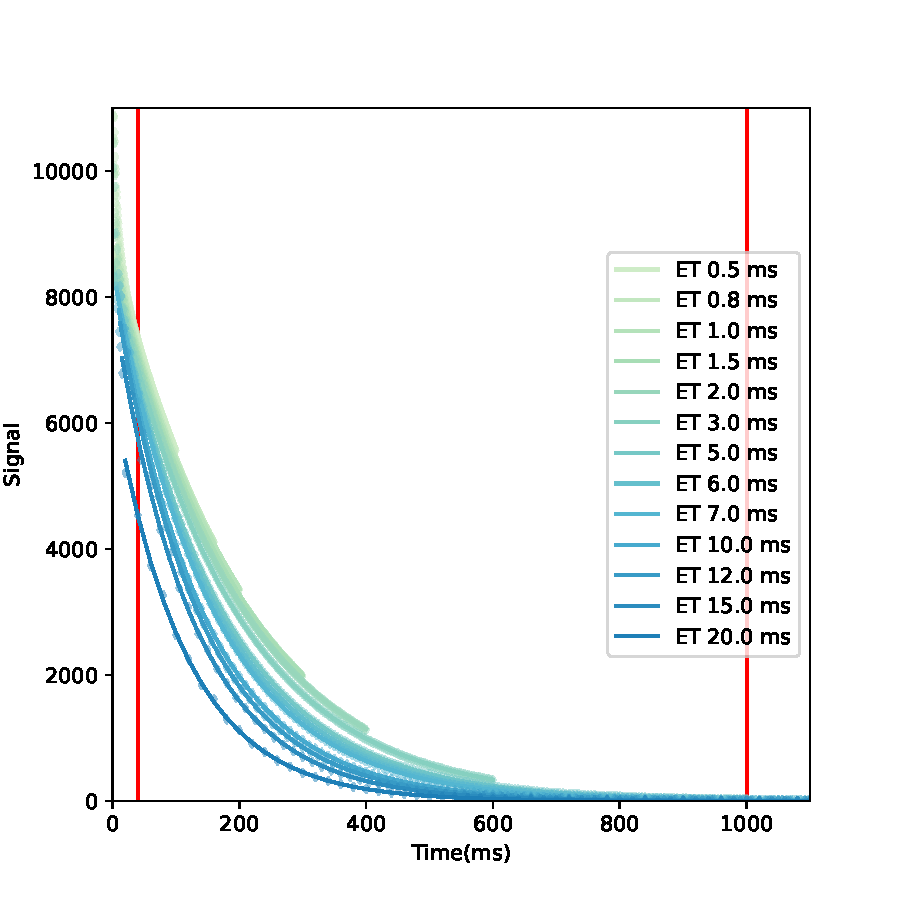
\includegraphics[width=10cm]{figures/diffmodels/20MHzT2fit.pdf}

\caption{CPMG decays measured at the field of 20 MHz, at the different echo times. Red lines indicate data points used for fitting}
\label{fig:dm-CPMGdecay}
\end{figure}

With the exception of the fast decay from the plastic tube at the start of the CPMG experiment, the log of the echo intensities follow a linear trend, which confirms that the blood is not separating, and that the decay is not significantly affected by the flow.

\subsection{Model fitting}

Values of \Ttwo measured at each echo time were then used as inputs for fitting equations \ref{eq:LMsimp} and \ref{eq:JC}.
Errors from the \Ttwo fitting are on the order of \SI{2}{ms}.
The resulting best fit curves for both equations are shown in \autoref{fig:dm-fitResults}, while the parameters are included in \autoref{tab:dm-fitPars}.

\begin{landscape}
\begin{table}[h]
\centering

\caption[Best fit values to the experimental data at different fields]{Best fit values to the experimental data at different fields, shaded columns indicate fixed parameters in fitting. Note that the \TtwoO values are going to be dependent on the state of the blood in the flow circuit, so are not necessarily reflective of the diffusion/exchange effects.}
\label{tab:dm-fitPars}


\makebox[\textwidth][c]{
\begin{tabular}{l|cccr|cccr|}
%Copied from Python/processCPMGvt/newCPMGvt
& \multicolumn{4}{c}{Constrained LM} & \multicolumn{4}{c}{Unconstrained LM} \\ Field 
& T\textsubscript{20} & K\textsubscript{0} & Tau\textsubscript{ex} \cellcolor[gray]{0.8} & SSR
& T\textsubscript{20} & K\textsubscript{0} & Tau\textsubscript{ex} & SSR\\
 & ms & 10\textsuperscript{-14} T\textsuperscript{2} & ms \cellcolor[gray]{0.8} & ms\textsuperscript{2}& ms & 10\textsuperscript{-14} T\textsuperscript{2} & ms & ms\textsuperscript{2}\\ \hline
40 MHz & 227 \pm 4.2 & 7.081 \pm 0.162 & 3.00 \cellcolor[gray]{0.8} & 3733 & 248 \pm 5.8 & 8.445 \pm 0.311 & 2.08 \pm 0.11 & 1199\\
20 MHz & 219 \pm 1.6 & 2.832 \pm 0.022 & 3.00 \cellcolor[gray]{0.8} & 277 & 210 \pm 1.9 & 2.459 \pm 0.048 & 3.55 \pm 0.08 & 498\\
14 MHz & 297 \pm 0.5 & 0.868 \pm 0.005 & 3.00 \cellcolor[gray]{0.8} & 410 & 298 \pm 0.5 & 0.990 \pm 0.020 & 2.30 \pm 0.08 & 183\\
10 MHz & 294 \pm 1.5 & 0.473 \pm 0.023 & 3.00 \cellcolor[gray]{0.8} & 616 & 305 \pm 3.3 & 0.654 \pm 0.062 & 1.96 \pm 0.18 & 89\\
5  MHz & 277 \pm 2.2 & 0.392 \pm 0.025 & 3.00 \cellcolor[gray]{0.8} & 443 & 283 \pm 3.2 & 0.588 \pm 0.092 & 1.81 \pm 0.30 & 177\\

%stop copying

\end{tabular}
}

\vspace{1cm}

\makebox[\textwidth][c]{
\begin{tabular}{l|cccr|cccr|}

%Same deal..
& \multicolumn{4}{c}{Constrained JC} & \multicolumn{4}{c}{Unconstrained JC} \\ Field 
& \TtwoO & \Gzero & \rc \cellcolor[gray]{0.8} & SSR
& \TtwoO & \Gzero & \rc & SSR\\
 & \si{ms} & \SI{e-14}{T^2} & \si{\micro\metre} \cellcolor[gray]{0.8} & \si{ms^2} & \si{ms} & \SI{e-14}{T^2} & \si{\micro\metre} & \si{ms^2}\\ \hline
40 MHz & 253 \pm 5.2 & 9.985 \pm 0.217 & 4.30 \cellcolor[gray]{0.8} & 844 & 272 \pm 8.6 & 11.643 \pm 0.636 & 3.58 \pm 0.19 & 120\\
20 MHz & 225 \pm 1.7 & 3.932 \pm 0.031 & 4.30 \cellcolor[gray]{0.8} & 56 & 220 \pm 2.4 & 3.588 \pm 0.105 & 4.65 \pm 0.12 & 34\\
14 MHz & 299 \pm 0.5 & 1.227 \pm 0.007 & 4.30 \cellcolor[gray]{0.8} & 88 & 300 \pm 0.6 & 1.393 \pm 0.044 & 3.70 \pm 0.12 & 35\\
10 MHz & 301 \pm 1.9 & 0.748 \pm 0.036 & 4.30 \cellcolor[gray]{0.8} & 181 & 309 \pm 4.4 & 1.022 \pm 0.161 & 3.29 \pm 0.38 & 13\\
5  MHz & 279 \pm 2.3 & 0.571 \pm 0.036 & 4.30 \cellcolor[gray]{0.8} & 302 & 291 \pm 5.7 & 1.364 \pm 0.485 & 2.32 \pm 0.48 & 34\\

%Stop thecopy
\end{tabular}
}
\end{table}
\end{landscape}

As expected, all of the curves show that longer echo times create a larger decrease in the \Ttwo.
Additionally, the magnitude of the effect becomes much weaker at lower field - for example, at 40 MHz the \Ttwo drops \SI{200}{ms} (from \SI{270}{ms} to \SI{70}{ms}) while at 10 MHz, the \Ttwo drop is \SI{60}{ms} (\SI{300}{ms} to \SI{245}{ms}).

The fitted curves show relatively good agreement with the experimental data, particularly in 20 MHz (b) and 14 MHz (c) and 10 MHz (d) experiments.
Generally, the unconstrained fits (solid lines) perform better than the constrained fits, this is shown again by the lower SSR values in \autoref{tab:dm-fitPars}.
This is expected due to the extra free parameter in the curve fitting procedure.

In the 40 MHz experiment, there is a larger deviation between the data points and best fit curves, particularly at short echo times.
The start of the curve is strongly influenced by the \TtwoO term, which reflects the intrinsic relaxation at infinitely short refocusing times (i.e. removing the effect of exchange or diffusion.)
This means that the  \TtwoO term may be underestimated in this experiment, which would also explain the larger uncertainty relative to the other field strengths.

The results also suggest that the diffusion model produces better agreement than the Luz Meiboom model.
This is shown by the decreased SSR in all cases, when comparing results at the same field strength.

The \TtwoO values tend to be between \SIrange{250}{310}{ms} for all except the 20 MHz experiments which are at \SI{220}{ms}.
This may be due to the state of the blood in the flow circuit, because as mentioned in \autoref{ch:cont}, experiments at 20 MHz were run after the 40 MHz, using the same blood sample.
This is unlikely to be correlated to the flow rate, as the 5 MHz results were measured at a similarly fast speed.

Additionally, trends can also be seen in the \Kzero and \Gzero values.
These values reflect the strength of the magnetic field inhomogeneities, which is dependent on the oxygen saturation, haematocrit and also on the magnetic field strength.
While this property was examined in \autoref{ch:cont}, to investigate the dependence on oxygen saturation, in these samples where oxygen saturation is uniformly low the \Kzero and \Gzero terms should have a dependence on the field strength.
The \Kzero and \Gzero values for the unconstrained fits follow a decreasing trend, although the \Gzero increases at the 5 MHz experiment, which may be related to the smaller \rc.
The values of \Kzero and \Gzero are plotted in \autoref{fig:dm-KGfield}, with a quadratic line of best fit plotted for the unconstrained \Kzero values. The resulting fit parameters give
 $\mathit{K_0=\num{8.56\pm0.34e-14}B_0^2}$ and $\mathit{G_0 = \num{11.8\pm0.7e-14}B_0^2}$.
\begin{figure}[h]
\centering
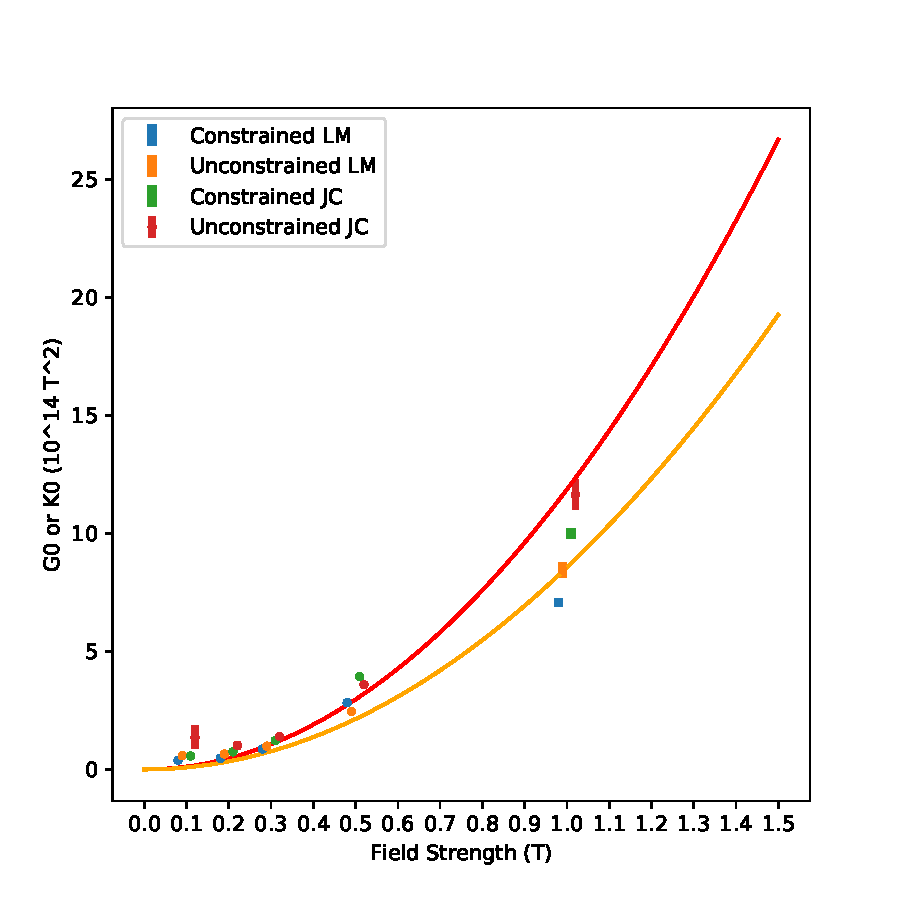
\includegraphics[width=10cm]{figures/diffmodels/G0K0field.pdf}
\caption[Field dependence of $G_0$ and $K_0$]{Field dependence of $G_0$ and $K_0$. Note points are moved on x-axis to better differentiate the series}
\label{fig:dm-KGfield}
\end{figure}

\begin{figure}[h!t]
  \makebox[\textwidth][c]{

  \begin{subfigure}[t]{0.6\textwidth}
  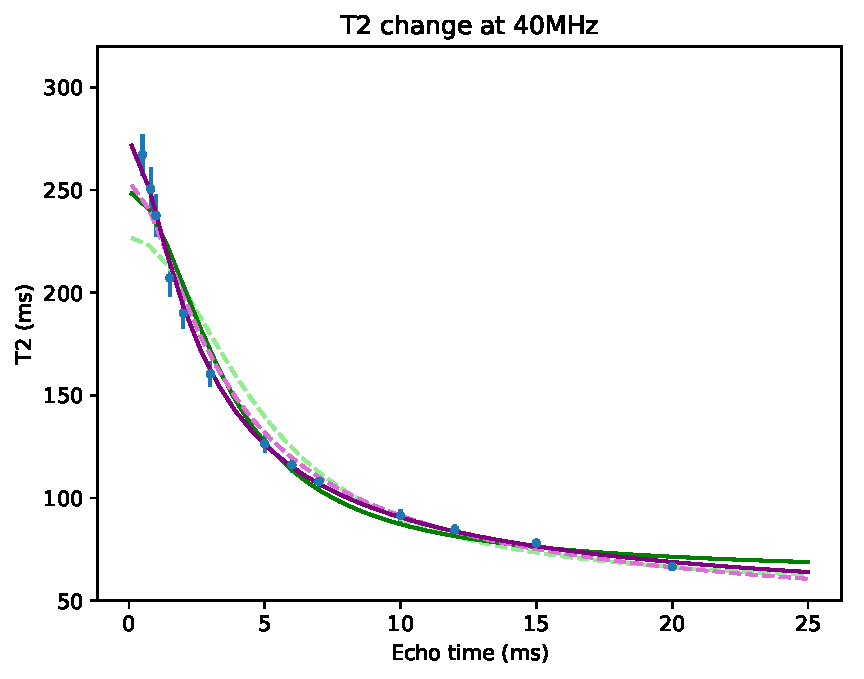
\includegraphics[width=\textwidth]{figures/diffmodels/40MHzT2.pdf}
  \caption{40 MHz: \SOtwo 2\%, Hct 0.35, v=1.0 cm/s}
  \label{fig:dm-fitResults40}
  \end{subfigure}
  \begin{subfigure}[t]{0.6\textwidth}
  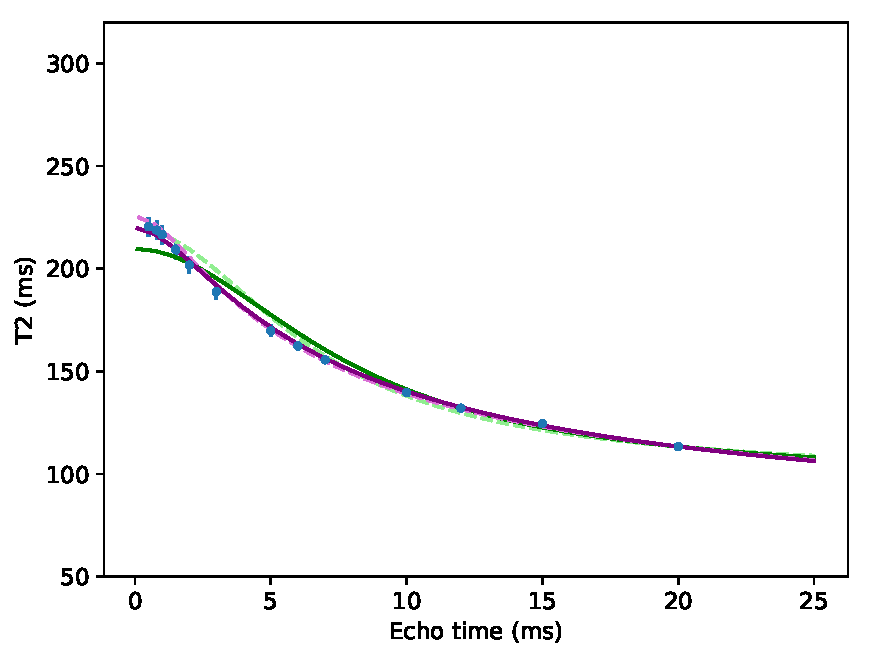
\includegraphics[width=\textwidth]{figures/diffmodels/20MHzT2.pdf}
  \caption{20 MHz: (\SOtwo 1\%, Hct 0.35, v=1.9 cm/s}
  \label{fig:dm-fitResults20}
  \end{subfigure}
  \hfill
  }

  \makebox[\textwidth][c]{
  \begin{subfigure}[t]{0.6\textwidth}
  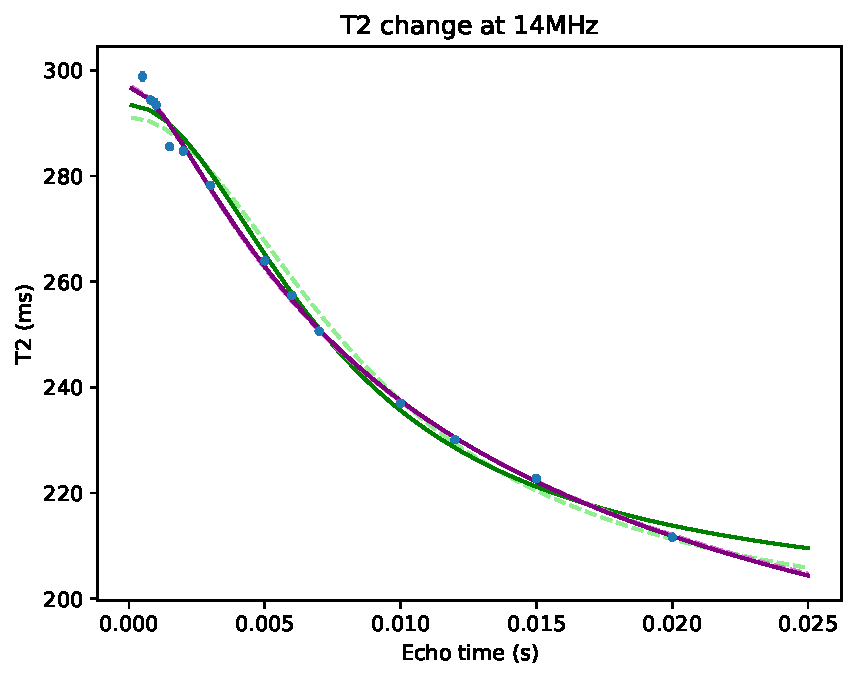
\includegraphics[width=\textwidth]{figures/diffmodels/14MHzT2.pdf}
  \caption{14 MHz: \SOtwo 5\%, Hct TODO iStat, v=1.1 cm/s}
  \label{fig:dm-fitResults14}
  \end{subfigure}
  \begin{subfigure}[t]{0.6\textwidth}
  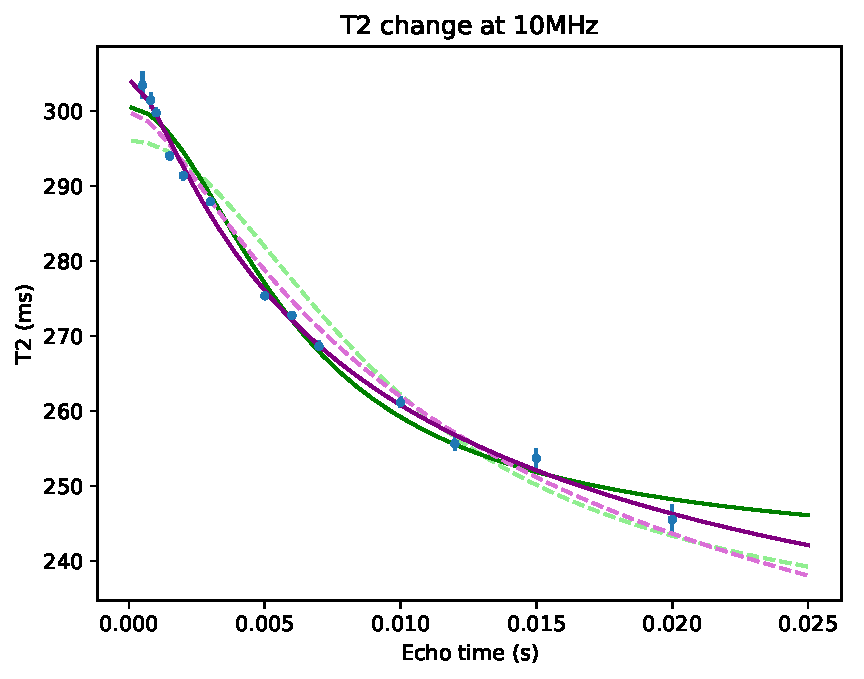
\includegraphics[width=\textwidth]{figures/diffmodels/10MHzT2.pdf}
  \caption{10 MHz: \SOtwo 2\%, Hct TODO iStat, v=1.6 cm/s}
  \label{fig:dm-fitResults10}
  \end{subfigure}
  \hfill
  }

  \makebox[\textwidth][c]{
  \begin{subfigure}[t]{0.6\textwidth}
  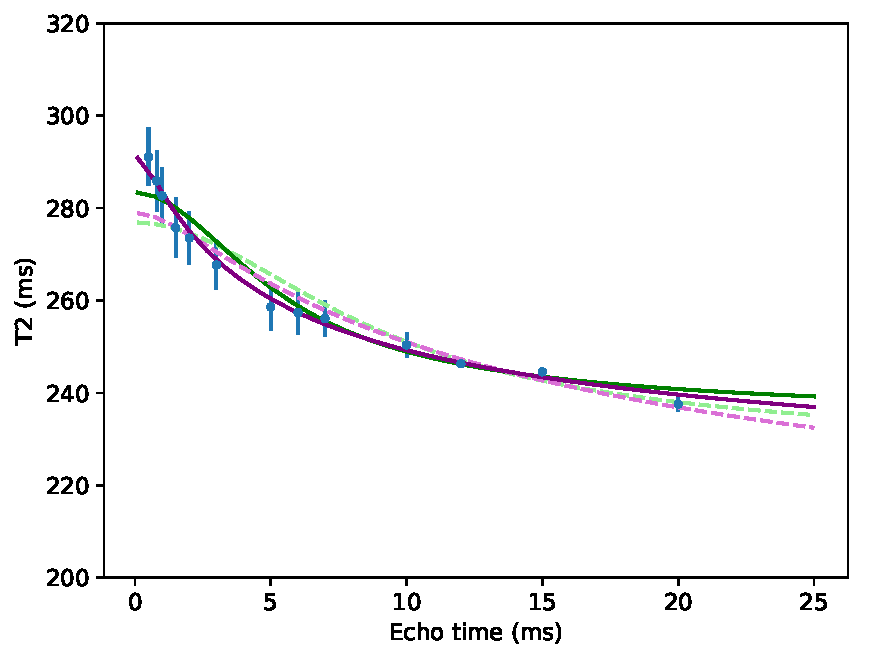
\includegraphics[width=\textwidth]{figures/diffmodels/5MHzT2.pdf}
  \caption{5 MHz: \SOtwo 7\%, Hct TODO iStat, v=2.5 cm/s}
  \label{fig:dm-fitResults5}
  \end{subfigure}
  \hspace{0.6\textwidth}
  }

  \caption[Luz-Meiboom and diffusion model fits at different fields]{Effect of changing echo time on \Ttwo at different fields, error bars show standard error (n=2). Best fit from Luz-Meiboom (Green) and diffusion model (Purple) are also shown. Dashed lines show constrained fits, while solid lines are unconstrained.}
  \label{fig:dm-fitResults}
\end{figure}

\section{Discussion}
These results show that the diffusion model of Jensen and Chandra tends to agree better with the measured data, even at low fields.
This is shown by the decreased SSR - the unconstrained JC fits provides much lower residuals than all other methods.
However, the curves / predictions of the LM model tend to be within \SI{10}{ms} of the experimental data, which means that both models are probably adequate for predicting \Ttwo.
This is the same conclusion reached by Stefanovic and Pike and Chen and Pike, who found that the Luz-Meiboom exchange model provides acceptable accuracy at 1.5 T and at 3T respectively.

Additionally, with the exception of the 20 MHz results (where experiments were run after the 40 MHz run), the unconstrained fits produce concordant results of \Texc = \SI{2.17\pm0.06}{ms} and \rc = \SI{3.58 \pm 0.08}{\micro\metre} (weighted mean across field strengths).
This value for \rc is within the range of red blood cell size, although it is smaller than the value found by Stefanovic (\SI{4.3}{\micro\metre})\cite{StefanovicHumanwholebloodrelaxometry2004}, and larger than the value found by Chen (\SI{2.7}{\micro\metre})\cite{ChenHumanwholeblood2009}.

This value for the exchange time is also within the range of results in the literature, although they do not correspond with the values measured at low field by Gomori\cite{GomoriNMRRelaxationTimes1987}.
This may be due to the long echo times they used, e.g. Gomori used two echo times of \SIlist{32}{64}{ms} at 0.94 T to get very short \Ttwo decays.
These long echo times were used because they were unable to get a good estimate of \Ttwo shortening at short echo times due to large uncertainties.
Looking at these long echo times may lead to greater sensitivity to exchange processes, and in particular, the \SI{9.1}{ms} exchange time found by Gomori aligns well with literature values from permeability studies of the red blood cell membrane, which found values on the order of \SI{10}{ms}\cite{Herbstreviewwaterdiffusion1989}.

Changes in the value of \rc when moving from 40 MHz to 20 MHz are interesting, as it is known to be the same sample of blood.
This could reflect changes in the state of the blood, due to being cycled through the flow circuit for 4 hours previously. TODO check how long??
More precisely, the fitted parameter in \autoref{eq:JC} is actually $\mathit{\frac{r_c^2}{2D}}$, and it is possible that an increase in the fitted \rc could also be due to a decrease in D, the diffusion coefficient.
While this data point is

The \Kzero and \Gzero terms tend to follow a quadratic curve, which agrees with the predictions of theory \cite[Eq. 52-54]{JensenNMRrelaxationtissues2000}.
Extrapolating this to 1.5 T predicts a value of \Gzero = \SI{26.7e-14}{T^2}.
This is about half of what is predicted using the results of Stefanovic, which (although based on studying changes in \SOtwo) can be used to find $\mathit{G_0} = \num{45\pm0.51e-14}  \mathit{(sO_2)^2} = \SI{40.6e-14}{T^2}$ when using \SOtwo = 0.03, the average value from our experiments.
While the difference is significant, it is important to note that the variation between the oxygenations and haematocrit used at the different field strengths was not taken into account when fitting the data to find \Gzero, and multiple researchers \cite{StefanovicHumanwholebloodrelaxometry2004,ChenHumanwholeblood2009,GardenerDependencebloodR22010} have found that these parameters are correlated.

One possible weakness to these results is the effect of flow on the \Ttwo measurements.
It was shown in previous TODO(section in continuousflow) that low amounts of flow through the circuit can cause slight decreases in the measured \Ttwo, without causing significant changes to the monoexponential decay in the CPMG experiment.
However, it is unclear whether the increasing echo time causes an increase in the strength of this effect, and whether it affects longer \Ttwo decays differently to shorter decays.
In these variable echo time experiments, this would be expected to cause underestimation \Ttwo values at longer echo times, which would lead to an overestimation in the magnitude of the \Ttwo shortening effect.
TODO find out the effect from water flow experiments??!!
While the models still provide good agreement with the data points, it is unclear how the blood velocity affects the accuracy of the fitting parameters, as flow rate varied from \SIrange{1}{2}{cm/s} between experiments.
Additionally, the flow rate has been assumed to be constant over the 5 minute course of the experiment.
This is relatively short compared to the longer term trends which were seen in the continuous flow experiments, so this should not have a significant effect.

As both models have acceptable predictions for the shape of the echo time curve, these results can not provide more evidence of the actual physical mechanism of the \Ttwo shortening effect.
To be able to determine this, other experimental NMR techniques would need to be used such as chemical shift exchange sensitive methods such as DDCOSY that could detect this process directly.
Other researchers have also used paramagnetic contrast agents to probe exchange between intra- and extracellular pools in blood\cite{LiIntegratedanalysisdiffusion1998}.
Matwiyoff \cite{Matwiyofflineshapeswater1990} proposed that as the field decreased below 1.5 T, the exchange time would increase as the mechanism moved from mainly diffusion to mainly exchange.
This is the opposite to the trend observed here, where there a slighty decreasing or constant trend in the exchange time, as field strength decreases.

Because of the variations between the measurements at different fields, with different samples of blood at each field, different amounts of time in the flow circuit, and variations in factors such as flow rate and oxygen saturation, it is difficult to make strong conclusions about the parameters underlying the models.
More data, with different samples of blood and better control of these experimental factors would need to be collected.
However, it is clear that both of the models are able to produce adequate agreement with experimental results.

\chapter{Conclusions}\label{ch:conc}

If all the economists in the world were laid end-to-end they wouldn't
reach a conclusion, and neither shall I.

\chapter*{Conference Attendance}
\label{ch:conference}
The work in this thesis was presented at:

\begin{itemize}
\item Y.C. Tzeng, \textbf{D.G. Thomas}, P. Galvosas, S. Obruchkov, P.D. Teal, Measurement of transverse relaxation properties of whole blood at low magnetic fields. The 14\textsuperscript{th} International Conference on Magnetic Resonance Microscopy, \textit{oral presentation}, Halifax NS Canada, August 2017
\item \textbf{Dion G. Thomas}, Petrik Galvosas, Yu-Chieh Tzeng, Paul D. Teal, Sergei Obruchkov, Measurement of transverse relaxation properties of whole blood at low magnetic fields. The 11\textsuperscript{th} Australian and New Zealand Society for Magnetic Resonance Conference, \textit{poster and short oral presentation}, Kingscliff NSW Australia, December 2017

\end{itemize}


%%%%%%%%%%%%%%%%%%%%%%%%%%%%%%%%%%%%%%%%%%%%%%%%%%%%%%%

% and of course book style knows about backmatter
% \backmatter caused problems with appendices :-(
% and of course report style doesn't
%%%%%%%%%%%%%%%%%%%%%%%%%%%%%%%%%%%%%%%%%%%%%%%%%%%%%%%


\bibliographystyle{ieeetr}
%\bibliographystyle{plain}
\bibliography{mscthesis}


\end{document}
